\documentclass[11pt,a4paper]{article}
\usepackage[margin=2.45cm]{geometry}
\usepackage{authblk}
\usepackage{caption}
\usepackage{float}
\usepackage[super,sort&compress]{natbib}
\setcitestyle{numbers,super}
\usepackage{amsmath,amssymb,amsfonts}
\usepackage{graphicx}
\usepackage{pdflscape}
\usepackage{pdfpages}
\usepackage{textcomp}
\usepackage{xcolor}
\usepackage{hyperref}

% Robust PDF bookmarks: keep acronym commands out of bookmark strings.
\pdfstringdefDisableCommands{%
  \def\ac#1{#1}%
  \def\acs#1{#1}%
  \def\acf#1{#1}%
  \def\acp#1{#1}%
  \def\Acp#1{#1}%
}
\usepackage{booktabs}
\usepackage{tabularx}
\usepackage{ragged2e}
\usepackage{array}
\usepackage{multirow}
\usepackage{microtype}
\usepackage[nohyperlinks]{acronym}
% Acronym definitions. Use \newacro in the preamble so acronyms are available on the first LaTeX pass.
% This avoids the acronym package's undefined-acronym fallback, which appears as bold text followed by an exclamation mark.
\renewcommand*{\aclabelfont}[1]{#1}
\newacro{AI}[AI]{artificial intelligence}
\newacro{HPC}[HPC]{high-performance computing}
\newacro{MLIP}[MLIP]{machine-learned interatomic potential}
\newacro{DFT}[DFT]{density functional theory}
\newacro{AL}[AL]{active learning}
\newacro{LLM}[LLM]{large language model}
\newacro{QE}[QE]{Quantum ESPRESSO}
\newacro{VASP}[VASP]{Vienna Ab initio Simulation Package}
\newacro{DOE}[DOE]{Department of Energy}
\newacro{NERSC}[NERSC]{National Energy Research Scientific Computing Center}
\newacro{OLCF}[OLCF]{Oak Ridge Leadership Computing Facility}
\newacro{ALCF}[ALCF]{Argonne Leadership Computing Facility}
\newacro{GNN}[GNN]{graph neural network}
\newacro{MLP}[MLP]{multilayer perceptron}
\newacro{MAE}[MAE]{mean absolute error}
\newacro{MC}[MC]{Monte Carlo}
\newacro{MD}[MD]{molecular dynamics}
\newacro{ASE}[ASE]{Atomic Simulation Environment}
\newacro{SOAP}[SOAP]{Smooth Overlap of Atomic Positions}
\newacro{FIRE}[FIRE]{Fast Inertial Relaxation Engine}
\newacro{BFGS}[BFGS]{Broyden--Fletcher--Goldfarb--Shanno}
\newacro{SCF}[SCF]{self-consistent field}
\newacro{RMS}[RMS]{root mean square}
\newacro{BCC}[BCC]{body-centered cubic}
\newacro{HEA}[HEA]{high-entropy alloy}
\newacro{GGA}[GGA]{generalized-gradient approximation}
\newacro{MOF}[MOF]{metal--organic framework}
\newacro{GPU}[GPU]{graphics processing unit}
\newacro{CUDA}[CUDA]{Compute Unified Device Architecture}
\newacro{MPI}[MPI]{Message Passing Interface}
\newacro{PVC}[PVC]{Ponte Vecchio}
\newacro{GCD}[GCD]{graphics compute die}
\newacro{NVT}[NVT]{constant-particle-number, constant-volume, constant-temperature}
\newacro{REPL}[REPL]{read--eval--print loop}
\newacro{JSON}[JSON]{JavaScript Object Notation}
\newacro{JSONL}[JSONL]{JavaScript Object Notation Lines}
\newacro{HTTP}[HTTP]{Hypertext Transfer Protocol}
\newacro{NLP}[NLP]{natural language processing}
\newacro{FFTW}[FFTW]{Fastest Fourier Transform in the West}
\newacro{ELPA}[ELPA]{Eigenvalue SoLvers for Petaflop-Applications}
\newacro{GTL}[GTL]{GPU transport layer}
\newacro{XPU}[XPU]{Intel accelerated processing unit}
\newacro{DFTB}[DFTB]{density-functional tight binding}
\newacro{GFM}[GFM]{graph foundation model}
\newacro{MTL}[MTL]{multi-task learning}
\newacro{MPNN}[MPNN]{message-passing neural network}
\newacro{ADIOS2}[ADIOS2]{Adaptable Input/Output System 2}
\newacro{DDStore}[DDStore]{Distributed Data Store}
\newacro{NVMe}[NVMe]{non-volatile memory express}
\newacro{FP64}[FP64]{64-bit floating point}
\newacro{FP32}[FP32]{32-bit floating point}
\newacro{BF16}[BF16]{bfloat16}
\usepackage{tikz}
\usetikzlibrary{shapes.geometric, arrows.meta, positioning, fit, backgrounds}

\def\BibTeX{{\rm B\kern-.05em{\sc i\kern-.025em b}\kern-.08em
    T\kern-.1667em\lower.7ex\hbox{E}\kern-.125emX}}


% Editorial revision markers, used ONLY for this author-facing draft.
\newcommand{\newexperiment}[2]{\par\medskip\noindent\begingroup\color{red!80!black}\textbf{NUMERICAL RESULTS PENDING: #1}\par\noindent\textbf{Evaluation:} #2\par\endgroup\medskip}
\newcommand{\verifyclaim}[1]{\par\smallskip\noindent{\color{red!80!black}\textbf{CLAIM / DATA TO VERIFY:} #1}\par\smallskip}
\newcommand{\revisionnote}[1]{\par\smallskip\noindent{\color{red!80!black}\textbf{REVISION NOTE:} #1}\par\smallskip}
\hypersetup{hidelinks}

\begin{document}
\title{MATSIM-AGENTS: A Multi-Backend Agentic Framework for Evidence-Grounded Atomistic Materials Characterization}
\author[1]{Massimiliano Lupo Pasini\thanks{Corresponding author: lupopasinim@ornl.gov}}
\author[2]{Zekun Chen}
\author[2]{Anubhav Jain}
\affil[1]{Computational Sciences and Engineering Division, Oak Ridge National Laboratory, USA}
\affil[2]{Energy Storage and Distributed Resources, Lawrence Berkeley National Laboratory, USA}
\date{}
\maketitle
\begin{abstract}
Scientific characterization of atomistic materials requires more than identifying plausible compositions or structures: it requires determining which physical claims are supported by numerical evidence, which remain unresolved, and which calculations can most efficiently reduce uncertainty. \acp{LLM} offer a flexible means of formulating hypotheses and coordinating investigations, whereas \acp{MLIP} and \ac{DFT} provide complementary levels of physical fidelity and computational cost. We present MATSIM-AGENTS, an open-source framework that couples hypothesis formulation and structured scientific assessment to atomistic structure generation, surrogate-model evaluation, first-principles calculations, and persistent computational workflows. The framework decouples scientific reasoning from numerical computation through modular backends, supporting MLIPs, including HydraGNN, Universal Models for Atoms (UMA), and Message Passing Atomic Cluster Expansion (MACE), as well as DFT calculations performed using the \ac{VASP} and Quantum ESPRESSO. Its scientific workflow distinguishes hypotheses from numerical predictions and higher-fidelity evidence, allowing computational results and their provenance to inform subsequent assessments and calculations. Initial materials campaigns illustrate integrated structure exploration, first-principles labeling, concurrent numerical execution, and resumption across computing allocations. The framework provides a basis for investigating whether evidence-conditioned reasoning improves the reliability and efficiency of atomistic characterization beyond conventional adaptive computational workflows.
\end{abstract}
\noindent\textbf{Keywords:} automated materials characterization; atomistic materials; large language models; machine-learned interatomic potentials; density functional theory; evidence-grounded reasoning; high-performance computing.
\par\bigskip
\acresetall

\section{Introduction}
\label{sec:intro}
The functional properties of materials are closely related to their chemical composition and atomistic structure. Understanding these relationships guides the design and selection of materials for targeted applications, from energy conversion and storage to catalysis and electronic devices. Atomistic calculations provide structural and energetic information that helps relate candidate compositions and configurations to their anticipated behavior. Computational characterization seeks to establish physical properties of these candidates through evidence obtained from numerical calculations. \Ac{DFT} provides electronic-structure-based energies, forces and structural information~\cite{hohenberg1964,kohn1965,kresse1996vasp,giannozzi2009qe}; \ac{MD} describes atomistic evolution with forces supplied by an interatomic potential or an electronic-structure method~\cite{verlet1967,car1985}. The computational expense of first-principles calculations constrains structural sampling, and different numerical observables support different scientific conclusions: a relaxed geometry or favorable energy ranking does not, by itself, establish thermodynamic stability against competing phases~\cite{ong2013pymatgen,sun2016metastability}. Characterization therefore requires both numerical evidence and an assessment of what the evidence justifies.

\Acp{MLIP} reduce the cost of repeated energy and force evaluations by learning from reference atomistic calculations. Foundational contributions include the high-dimensional neural-network potentials of Behler and Parrinello~\cite{behler2007}, Gaussian approximation potentials~\cite{bartok2010}, and deep-potential molecular dynamics~\cite{zhang2018deepmd}. Representations respecting physical symmetries, including smooth overlap of atomistic positions and symmetry-adapted learning~\cite{bartok2013soap,grisafi2018,musil2021}, helped establish the basis for geometrically constrained models. Tensor Field Networks and equivariant neural-network tools developed by Smidt and collaborators~\cite{thomas2018tfn,geiger2022e3nn}, together with SchNet, NequIP and Message Passing Atomic Cluster Expansion (MACE)~\cite{schutt2018,batzner2022,batatia2022}, advanced atomistic representation learning. Broad-domain models such as M3GNet, CHGNet, MACE-MP and Universal Models for Atoms (UMA) extend the range of pretrained potentials~\cite{chen2022m3gnet,deng2023,batatia2023macemp,wood2025uma}. Their predictive reliability nevertheless remains dependent on training coverage, reference-data fidelity and the specific physical quantity being inferred; pretraining alone cannot certify accurate predictions for an unfamiliar composition or structural environment.

\Acp{LLM} provide a different capability: they can formulate candidate scientific hypotheses, synthesize domain knowledge and organize computational investigations. Coscientist and SciAgents exemplify tool-supported scientific planning and multi-agent hypothesis formulation~\cite{boiko2023coscientist,ghafarollahi2025sciagents}. These capabilities do not turn language-generated hypotheses into quantitative physical evidence. A plausible explanation may conflict with numerical observations, and an incomplete or failed calculation may leave the scientific question unresolved. The difficulty is thus not only to execute a requested tool, but also to identify which observables are relevant, evaluate the strength of their support and decide what additional calculation is informative.

Materials-science LLM agents now span several complementary tasks. HoneyComb combines a curated materials knowledge base with a tool hub and adaptive retrieval~\cite{zhang2024honeycomb}; ChatMOF uses an agent, toolkit and evaluator for MOF retrieval, property prediction and structure generation~\cite{kang2024chatmof}; and MatSciAgent presents modular LLM agents for multi-task computational materials science~\cite{chaudhari2026matsciagent}. Other scientific workflow and agentic systems address complementary portions of the problem: MISPR automates prescribed density-functional and molecular-simulation workflows with provenance and error handling~\cite{atwi2022mispr}; ChemGraph supports language-model-driven chemical tool orchestration and benchmarks computational task completion~\cite{chemgraph2026}; and El Agente Potente emphasizes structured, reproducible atomistic execution~\cite{potente2026}. MASTER and MAESTRO couple agentic reasoning to numerical calculations in catalyst discovery and optimization~\cite{master2026,maestro2026}. These contributions establish important precedents in materials-science agents, workflow automation and computational discovery. The narrower question evaluated here is whether language-model-guided interpretation and follow-up calculation selection improve characterization reliability or efficiency relative to a capability-matched adaptive numerical workflow using the same computational methods.

Unlike materials discovery or optimization, where the objective is to identify candidates with desirable properties, materials characterization focuses on establishing the physical properties and behavior of a given material. This process often requires combining complementary computational methods, evaluating the reliability of their predictions, and determining whether the available numerical evidence is sufficient to support a scientific conclusion. These considerations motivate computational approaches capable of coordinating atomistic simulations with the formulation and assessment of scientific hypotheses.

We introduce \textsc{matsim-agents}~\cite{osti-code-181158}, an open-source agentic framework for automated atomistic materials characterization that integrates scientific hypothesis formulation, numerical simulation, and evidence-informed assessment within an iterative computational workflow. Scientific hypotheses guide the selection of atomistic calculations, while the resulting numerical evidence informs subsequent assessments and the identification of additional characterization needs. By connecting language-model reasoning with learned interatomic potentials and first-principles electronic-structure calculations, the framework supports systematic investigations of candidate compositions and atomistic configurations.

The framework separates three independently configurable classes of backend. LLM providers support hypothesis formulation and review; MLIP backends, including HydraGNN, UMA and MACE, support approximate atomistic energy and force evaluation; and DFT backends, including the \ac{VASP} and Quantum ESPRESSO, execute electronic-structure calculations. This separation preserves the different scientific responsibilities of the methods and permits alternative numerical implementations to be considered within a common characterization process. Persistent campaign records and execution mechanisms for heterogeneous \ac{HPC} systems connect evidence-based decisions to calculations that may span multiple computing allocations. While previous studies have explored the integration of \acp{LLM} with scientific computing tools, MATSIM-AGENTS brings together scientific hypothesis formulation, atomistic simulations, and evidence-informed hypothesis revision within a unified computational framework. By integrating \acp{MLIP}, \ac{DFT} calculations, and active learning, the framework enables scientific hypotheses to be investigated and progressively refined using numerical evidence of different levels of fidelity.

The reasoning interface is deliberately separable from the model's hosting environment: the same scientific prompt and evidence contract can be used with an institutionally operated open-weight model or a remotely served frontier model. These options are complementary rather than hierarchically interchangeable. Local serving can provide greater institutional control over checkpoint, software, telemetry and data paths where licensing and deployment permit, and can reduce the need to transmit prompts to an external provider; it is not inherently more scientifically capable, private, compliant or inexpensive. Remote services may offer competitive or stronger capabilities and reduce checkpoint and serving-infrastructure burden, but introduce service charges, network and provider dependencies, rate limits, model revisions or retirement, and less infrastructure visibility. Capability differences are empirical, and a comparison of model groups cannot attribute an observed quality difference to hosting location alone. For either deployment, data use requires institutional authorization and appropriate technical and contractual controls.

The scientific question evaluated in this work is whether that integration yields more reliable or efficient characterization than appropriate non-agentic alternatives. In particular, the evaluation distinguishes interpretation of previously computed evidence from live selection and execution of calculations, and compares language-model-guided decisions with capability-matched deterministic adaptive workflows. Independent comparisons across MLIP backends, physical reference calculations and computational platforms address predictive reliability and implementation scope. The following sections present the methodology, test cases and numerical setup, the three stages of numerical results, and conclusions and future work.

\section{Methodology}
\label{sec:architecture}

\begin{table}[htbp]
\centering
\caption{Comparison of MISPR, a pre-LLM automated materials-characterization framework, with representative recent agentic frameworks for atomistic science. Entries summarize the documented capabilities and the \emph{limits of what the published evaluations establish}, not an audit asserting that unreported capabilities are absent. ``To validate'' indicates a MATSIM-AGENTS capability present in the architecture for which stronger end-to-end or controlled experimental support is needed. DFT and MLIP denote density functional theory and machine-learned interatomic potential, respectively.}
\label{tab:agentic_comparison}
\scriptsize
\setlength{\tabcolsep}{4pt}
\renewcommand{\arraystretch}{1.06}
\begin{tabularx}{\textwidth}{@{}>{\RaggedRight\arraybackslash}p{0.15\textwidth}>{\RaggedRight\arraybackslash}p{0.21\textwidth}>{\RaggedRight\arraybackslash}X >{\RaggedRight\arraybackslash}p{0.24\textwidth}@{}}
\toprule
\textbf{Framework} & \textbf{Scientific objective / emphasis} & \textbf{Documented agent and scientific-computing capabilities} & \textbf{Reported evaluation boundary relevant to characterization} \\
\midrule
MISPR~\cite{atwi2022mispr} (non-agentic baseline) & High-throughput multiscale molecular and materials characterization & Automated Gaussian DFT and LAMMPS MD; FireWorks orchestration, error correction, property analysis, persistent results databases and provenance. No LLM reasoning layer is described. & Limitation for this research question: documented workflows do not incorporate an LLM hypothesis-assessment/revision layer; they automate prescribed numerical tasks. This is a design scope, not a deficiency in numerical reliability. \\
\addlinespace
ChemGraph~\cite{chemgraph2026} & General computational chemistry and materials-simulation assistance & LLM task planning, multi-agent decomposition, scientific calculator access, and benchmarked task completion across 13 tasks. & Published benchmark assesses computational task completion, not the full DFT-label $\rightarrow$ MLIP-adaptation $\rightarrow$ independent-test $\rightarrow$ hypothesis-revision sequence. Unreported does not mean unsupported. \\
\addlinespace
El Agente Potente~\cite{potente2026} & High-throughput MLIP-based atomistic simulation and configurable workflows & Typed execution graphs, deterministic numerical tools, provenance-aware execution, alternative coding-agent mode; reproducibility and token-cost evaluation. & Published emphasis is auditable simulation and workflow reproducibility; integrated adaptation using newly acquired DFT data and externally scored characterization conclusions are not established as general benchmark outcomes. \\
\addlinespace
MASTER~\cite{master2026} & Hierarchical reasoning for catalyst discovery & LLM design/review strategies coupled to validated DFT and evaluated against agentic and heuristic baselines. & Evaluation is centered on catalyst-search performance and simulation efficiency; general characterization completeness, scientific abstention and three-layer backend substitution are not the measured objectives. \\
\addlinespace
MAESTRO~\cite{maestro2026} & Iterative single-atom catalyst optimization & Specialized design, calculation, reflection, and history-summary agents; simulation-informed candidate modification. & Published objective is optimization of single-atom catalysts; a task-independent characterization benchmark and interchangeable DFT/MLIP/LLM validation are outside its reported primary evaluation. \\
HoneyComb~\cite{zhang2024honeycomb} & Materials-science knowledge retrieval and tool use & Curated materials knowledge base, materials tool hub, and adaptive retrieval across knowledge and tools. & Evaluates materials-science tasks; the present capability-matched characterization comparison is a distinct question. \\
ChatMOF~\cite{kang2024chatmof} & MOF retrieval, property prediction, and structure generation & Agent, toolkit, and evaluator for natural-language-driven MOF tasks. & Evaluates retrieval, prediction, and generation; not the capability-matched characterization comparison studied here. \\
MatSciAgent~\cite{chaudhari2026matsciagent} & Multi-task computational materials science & Modular LLM agents for computational materials-science tasks. & Addresses a distinct task suite; this work evaluates iterative characterization against a matched adaptive numerical policy. \\
\addlinespace
\textbf{MATSIM-AGENTS (this work)} & \textbf{Automated atomistic materials characterization as a foundation for discovery} & Configurable LLMs, HydraGNN/UMA/MACE MLIPs, VASP/QE DFT interfaces; MLIP exploration, labeling, fine-tuning, structured evidence review, persistent execution, and HPC deployment. & Reported: unattended Perlmutter campaigns, numerical labeling throughput, allocation-boundary restart. \textbf{To validate:} independent-test decisions, agent value, complete backend substitution, and cross-facility numerical execution. \\
\bottomrule
\end{tabularx}
\end{table}


Facility-specific execution and resource placement are described in Appendix~\ref{sec:hpc}. Backend interoperability, throughput, restart behavior, and computational-cost accounting are detailed in Appendix~\ref{sec:appendix:performance}.

\subsection{Scientific objectives and framework architecture}

\paragraph{Implementation and data contracts.}
The scientific objective is made executable through a versioned, schema-validated \texttt{CharacterizationContract} (\texttt{matsim\_agents.campaign.characterization}), which declares the objective, input structures, requested observables and units, minimum admissible evidence level, numerical tolerances, method settings, reference data, resource budget and approval requirements. The executable command \texttt{matsim-agents characterize CONTRACT.yaml} dispatches a deterministic recipe for \texttt{relaxation}, \texttt{energy\_ranking}, or \texttt{thermodynamic\_stability}. The planner produces an ordered calculation graph, but physical observables are computed by the relaxation and stability operators rather than generated by language models. Results are returned as typed \texttt{CharacterizationReport} objects with an explicit status, recorded observables, evidence identifiers and missing requirements. A contract that cannot be satisfied is not converted into a positive scientific conclusion: invalid protocols, unsuccessful infrastructure, or insufficient evidence lead to correspondingly qualified reports. The execution fingerprint incorporates input structures and reference-file contents; operational changes such as budget increases or approval of an outstanding calculation can resume the existing scientific problem, whereas changed scientific inputs require a different execution state.

\paragraph{Capability-aware numerical dispatch.}
Backend support is represented in \texttt{matsim\_agents.execution.capabilities}, which records supported tasks, evidence levels, uncertainty or adaptation support, and runtime requirements. The \texttt{matsim-agents capabilities check} and \texttt{capabilities matrix} interfaces test local availability and expose supported configurations. These checks identify usable software installations; they do not imply numerical equivalence between different electronic-structure methods or certification of every model--facility combination.
\textsc{matsim-agents} is structured around three layers:
(i) a \emph{natural language interface} layer accepting free-text objectives
or interactive chat; (ii) a \emph{LangGraph orchestration layer} implementing
the multi-agent graph; and (iii) an \emph{atomistic backend layer} providing
\ac{MLIP} relaxation, stability scoring, and \ac{DFT} execution. The architecture separates task interpretation, numerical evidence generation, and scientific assessment. The subsections that follow specify the software contracts of each layer; the separate evidence-cycle diagram in Section~\ref{sec:results_phase} focuses more narrowly on the scientific meaning of hypothesis assessment after numerical evidence has been collected.
Figure~\ref{fig:architecture} provides an integrated view of the workflow, the configurable backend families, and the reproducibility and portability services that support execution. The top portion summarizes how composition hypotheses are proposed, tested, revised, and, when needed, escalated to higher-fidelity calculations; the lower portion summarizes representative \ac{LLM}, \ac{MLIP}, and \ac{DFT} backend options together with the state-management and cross-facility services that make those choices interchangeable at the workflow level.

A deliberate boundary separates what the \ac{LLM} decides from what the
explicit scientific-computation stages compute. The \acp{LLM} translate a
free-text objective into a typed plan, select which tool to run next, branch on
measured evidence, and produce human-readable summaries. The \acp{LLM} are used for
plan translation, tool selection, conditional branching, state tracking, failure
recovery, and natural-language explanation of workflow decisions.
 The
\acp{LLM} do not replace physical models or numerical solvers.
All physical quantities are
produced by explicit scientific codes and numerical models---\ac{ASE} relaxation
and \ac{MD}, \ac{MLIP} and \ac{DFT} evaluations, the backend training scripts,
and Slurm-scheduled jobs.

\clearpage
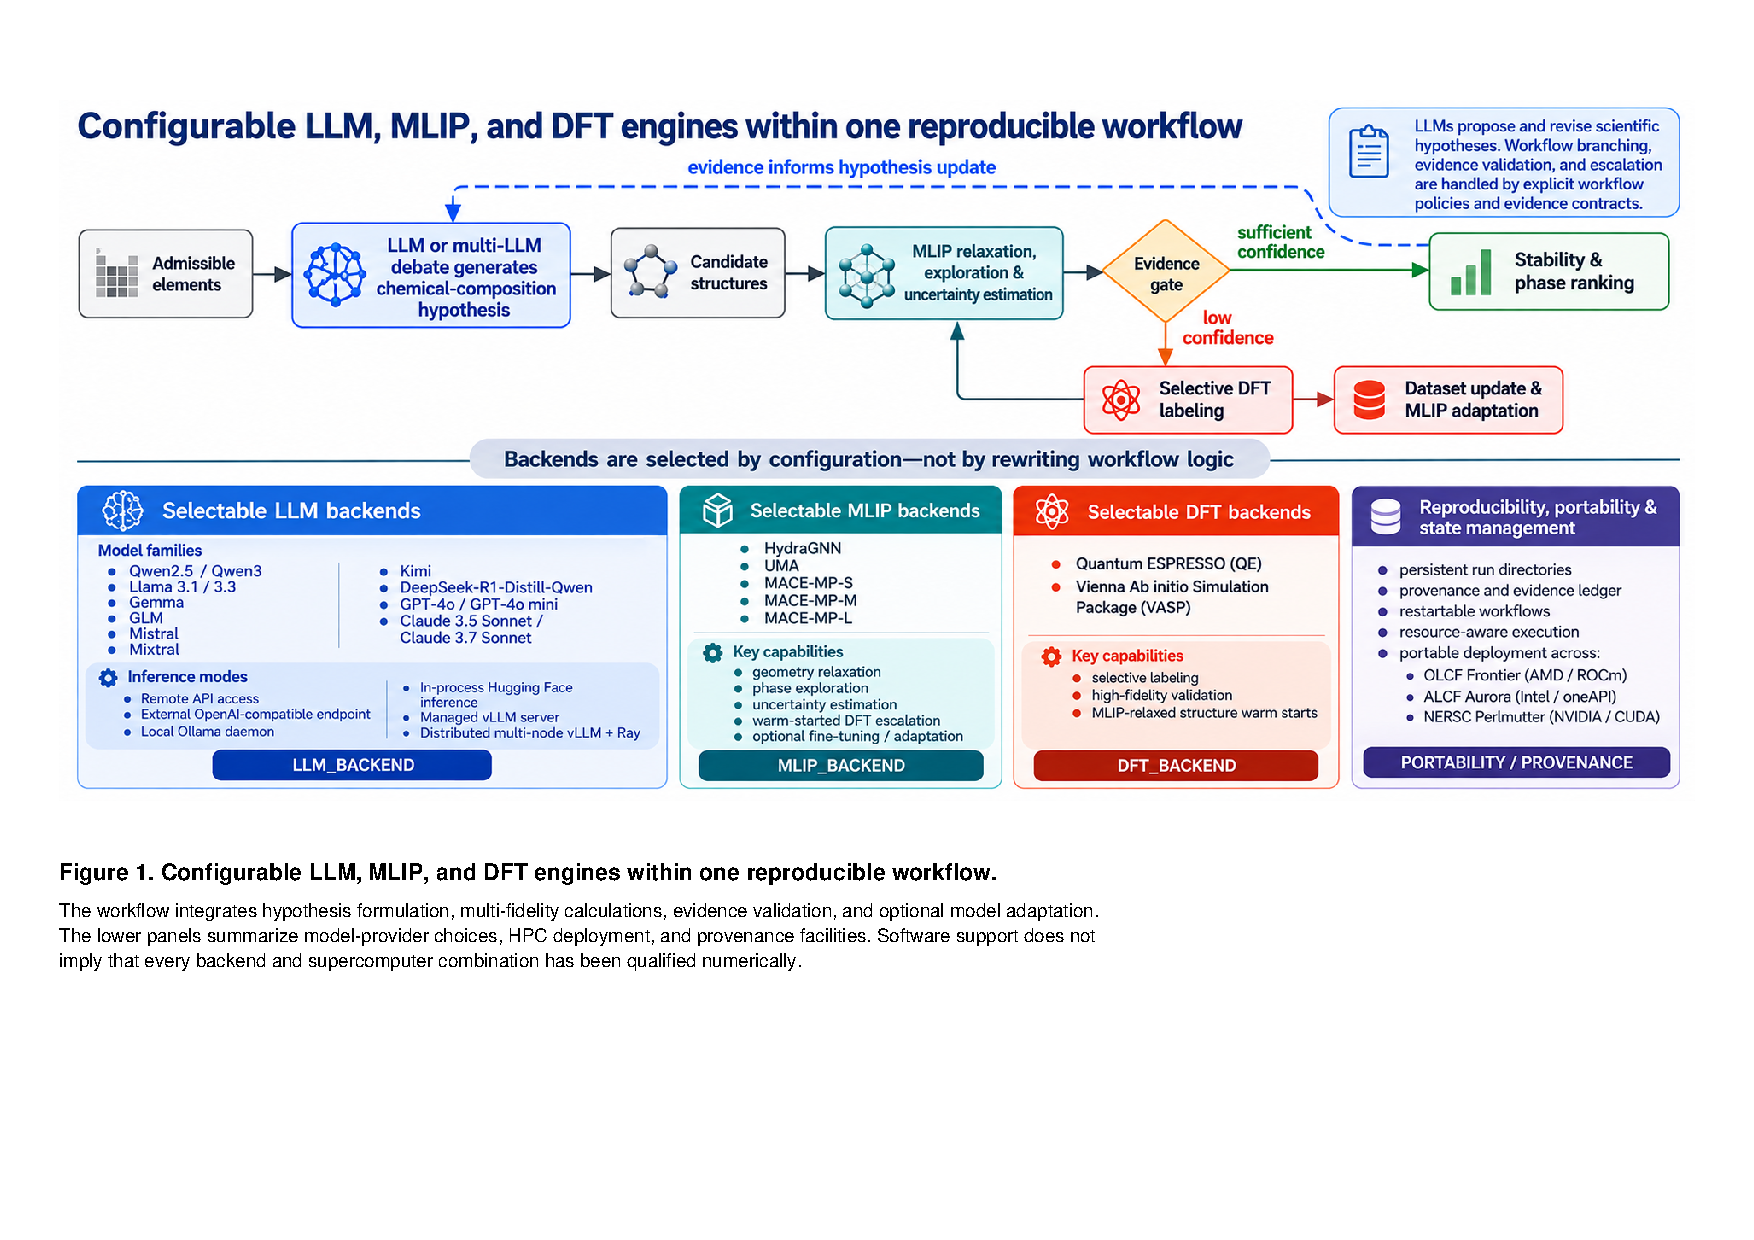
\includepdf[pages=1,fitpaper=true,pagecommand={\refstepcounter{figure}\label{fig:architecture}}]{figures/fig_architecture_A4_landscape.pdf}
\clearpage

\subsection{Scientific hypothesis formulation and multi-LLM debate}

\subsubsection{Language-model access, local serving and distributed inference}
\label{sec:methods:llm_deployment}
The language-model reasoning layer supports two deployment strategies. In the first, a model is accessed remotely through a provider-hosted application programming interface (API), with authentication supplied by an API key. The provider abstraction in \texttt{matsim\_agents.backends.llm.provider} constructs LangChain-compatible clients for the hosted OpenAI and Anthropic services. An independently operated OpenAI-compatible endpoint can also be used, including a model server reachable from the HPC facility; in this case the endpoint address and, when required, an authentication token are supplied through configuration rather than model weights being loaded in the application process. Remote access therefore separates the scientific workflow from the location and accelerator resources used for inference. Provider availability and outbound-network policies must be checked for the actual computing environment.
These implemented access paths are summarized visually in the lower-left panel of Figure~\ref{fig:architecture}, which also clarifies that local serving and distributed inference are treated as configurable deployment choices rather than as changes to the scientific workflow itself.

In the second strategy, the weights of a locally deployable model are obtained in advance and stored in a directory accessible to the allocated HPC compute nodes, typically on a facility parallel file system. Model licensing and access conditions remain those imposed by the model distributor; a locally downloadable model is not necessarily open-source. The framework provides three distinct local inference interfaces. The \texttt{huggingface} provider uses \texttt{transformers} through \texttt{langchain\_huggingface} and Hugging Face Accelerate, loading a model directly into the application process from \texttt{MATSIM\_HF\_MODEL\_PATH} or a configured model path. Its \texttt{device\_map="auto"} placement can partition weights over multiple GPUs visible to that process, subject to memory bounds imposed by the resource plan. This is an \emph{in-process, single-node} model-loading path in the current resource-placement implementation; it should not be conflated with distributed inference spanning several compute nodes. The \texttt{ollama} provider communicates with a locally running Ollama daemon through its configured HTTP endpoint (\texttt{MATSIM\_OLLAMA\_BASE\_URL}). The \texttt{vllm} provider instead sends OpenAI-compatible requests to a vLLM inference server (\texttt{MATSIM\_VLLM\_BASE\_URL}); the Python client does not load the model weights in this case.

For managed local serving, \texttt{matsim\_agents.execution.placement} describes named \texttt{external}, \texttt{in-process}, or \texttt{managed-vllm} model endpoints and assigns nodes, accelerator indices, device-memory budgets and, when appropriate, a tensor-parallel size. The \texttt{matsim\_agents.backends.llm.servers.VLLMServerManager} starts configured vLLM servers on their allocated resources, checks readiness through the \texttt{/v1/models} endpoint and cleans up server processes after use. When a model exceeds the capacity of a single accelerator, vLLM tensor parallelism partitions the model computation across multiple devices. For multi-node serving, the facility launchers start a Ray head on the serving node and Ray workers on other allocated nodes, expose the selected devices through accelerator masks, and launch \texttt{vllm serve} with \texttt{--distributed-executor-backend ray}. The implementation also accepts a pipeline-parallel setting where specified. The launchers use Slurm/\texttt{srun} on Frontier and Perlmutter and PBS Pro/\texttt{mpiexec} on Aurora; the scientific agents communicate with the resulting inference service through the same model endpoint regardless of its distributed placement. Facility-specific GPU communication libraries and process-launch settings remain part of the execution environment, rather than of the scientific reasoning algorithm.

The orchestration layer can assign different named inference servers to the proposer and reviewer roles, including mixtures of remotely hosted and locally served models. Consequently, the multi-LLM debate protocol is independent of whether each participant is accessed through a commercial API, an external server, a local daemon, or a locally managed distributed vLLM instance. For reproducibility, report the provider and exact model identifier; record a checkpoint revision or hash for local weights and provider-exposed model/version and request metadata for hosted APIs. Also report endpoint class, decoding settings, context and token limits, number and type of allocated accelerators, and model-serving parallelism. Where a model requires several nodes, serving cost must include all reserved nodes and accelerators rather than only the client process.

\begin{table}[htbp]
\centering
\caption{Considerations when selecting local open-weight and remotely served frontier LLMs. The entries describe potential operational characteristics, not universal guarantees or measured rankings; specific models, licenses, institutions and providers differ.}
\label{tab:llm_deployment_comparison}
\scriptsize
\setlength{\tabcolsep}{4pt}
\renewcommand{\arraystretch}{1.08}
\begin{tabularx}{\textwidth}{@{}>{\RaggedRight\arraybackslash}p{0.19\textwidth}>{\RaggedRight\arraybackslash}X>{\RaggedRight\arraybackslash}X@{}}
\toprule
\textbf{Dimension} & \textbf{Locally hosted open-weight models} & \textbf{Remotely served frontier models} \\
\midrule
Scientific reasoning capability & Depends on checkpoint, training, tools and task; local hosting is not evidence of greater scientific quality. & May provide stronger or complementary capabilities; superiority for these tasks is an empirical question, not assumed. \\
Availability & Subject to license, checkpoint access, storage, and compatible local hardware/software. & Subject to provider, account, network, regional and service availability. \\
Confidentiality and data sovereignty & Can reduce external prompt transfer and increase control of data paths, if the full deployment is institutionally approved. Local execution alone does not guarantee privacy, compliance, or authorization for classified, controlled, or restricted data. & Prompts are transmitted to a provider; before nonpublic data are sent, institutional approval, applicable governance, retention/training terms, access controls, and contractual protections must be checked. \\
Reproducibility & Exact checkpoint and serving stack may be pinned and archived when permitted; hardware and kernels can still affect outputs. & Record provider, exact model identifier, API settings, timestamp/version where exposed, and returned metadata; provider-side changes may limit replay. \\
Checkpoint and software control & Greater control over weights, inference software, logging and telemetry where the license and deployment allow; requires maintaining the stack. & Provider manages weights and infrastructure; users generally have less visibility and control over serving implementation and telemetry. \\
Startup and deployment complexity & Requires checkpoint acquisition, compatible software, storage, accelerator placement, serving and maintenance. & Usually lower model-serving setup burden, but requires credentials, network connectivity, service configuration and governance review. \\
Cost basis & Not free: charge or opportunity cost includes HPC allocation, accelerators, energy, storage, engineering, and ongoing maintenance; utilization and amortization matter. & API/token or subscription charges, plus integration, network and monitoring costs; prices and terms can change. \\
Latency and throughput & Depends on queueing, allocation, model size, batching and local load; dedicated serving may improve throughput but reserves resources. & Depends on network, provider load, limits, batching options and service tier; elastic capacity is not guaranteed. \\
Long-context support & Limited by checkpoint and serving configuration, available memory and throughput. & Limited by the selected model and API tier; advertised context is not necessarily effective scientific context. \\
Availability and rate limits & Constrained by allocation, hardware contention, maintenance and local service capacity. & Subject to provider outages, quotas, rate limits, regional access and network policy. \\
Retirement and preservation & A permitted checkpoint and its dependencies may be preserved locally, subject to storage, license and reproducibility constraints. & Model identifiers can be revised or retired; preserve permitted request/response records and version metadata, not provider weights. \\
Government-laboratory suitability & May support approved controlled data paths, but suitability depends on authorization, access, network, logging, storage, provenance and supply-chain review. & Use with nonpublic data only under applicable institutional approval and provider terms; remote location or a government-lab account does not by itself establish suitability. \\
\bottomrule
\end{tabularx}
\end{table}
The table motivates an empirical comparison of deployment approaches, not a claim that hosting environment is an isolated causal treatment. Model capability, training data, context window, decoding, serving implementation and version are coupled to the available deployment; these factors must be reported and considered when interpreting group differences.

\paragraph{Reasoning implementation and recorded decisions.}
LLM access is separated from scientific operators by \texttt{matsim\_agents.backends.llm.provider}, while hypothesis debate and review are implemented through \texttt{matsim\_agents.workflows.debate} and \texttt{matsim\_agents.campaign.review}. Structured reviewer outputs distinguish the scientific claim, its proposed test, the evidence being considered, and a proposed assessment. For campaign review, the evidence shown to reviewers includes numerical method, fidelity, convergence, reference completeness and persistent evidence identifiers. Reviewers must cite those identifiers when proposing a change to a hypothesis or a consequential candidate decision. Proposed revisions are checked before being appended to the evidence history; rejected proposals are retained as rejected review output rather than silently becoming accepted scientific findings. This records \emph{what the reasoning layer proposed} separately from \emph{what the numerical evidence permits}.

A separate evaluation operator, \texttt{matsim\_agents.campaign.agent\_eval}, supports matched-budget assessment of reasoning configurations on structured claim--evidence problems. Its cases include supported and contradicted claims, missing evidence, unsuccessful calculations, incomplete reference sets and disagreements between computational protocols. These cases test admissibility and reasoning behavior; their representative fixture values should not be presented as independent first-principles calculations.
The first two layers, the natural-language interface
and the LangGraph orchestration layer, are realized together by a single
multi-agent graph and the entry points that expose it to the user.

The conditional execution pathways and the distinction between uncertainty-driven DFT acquisition, evidence sufficiency, scientific hypothesis revision, and model promotion are illustrated in Figure~\ref{fig:agentic_scientific_workflow}. The three user-facing modes share scientific operators, while characterization contracts and evidence-ledger checks apply only to the workflows for which they are configured. In particular, MLIP adaptation is a separate feedback path from hypothesis revision.

\clearpage
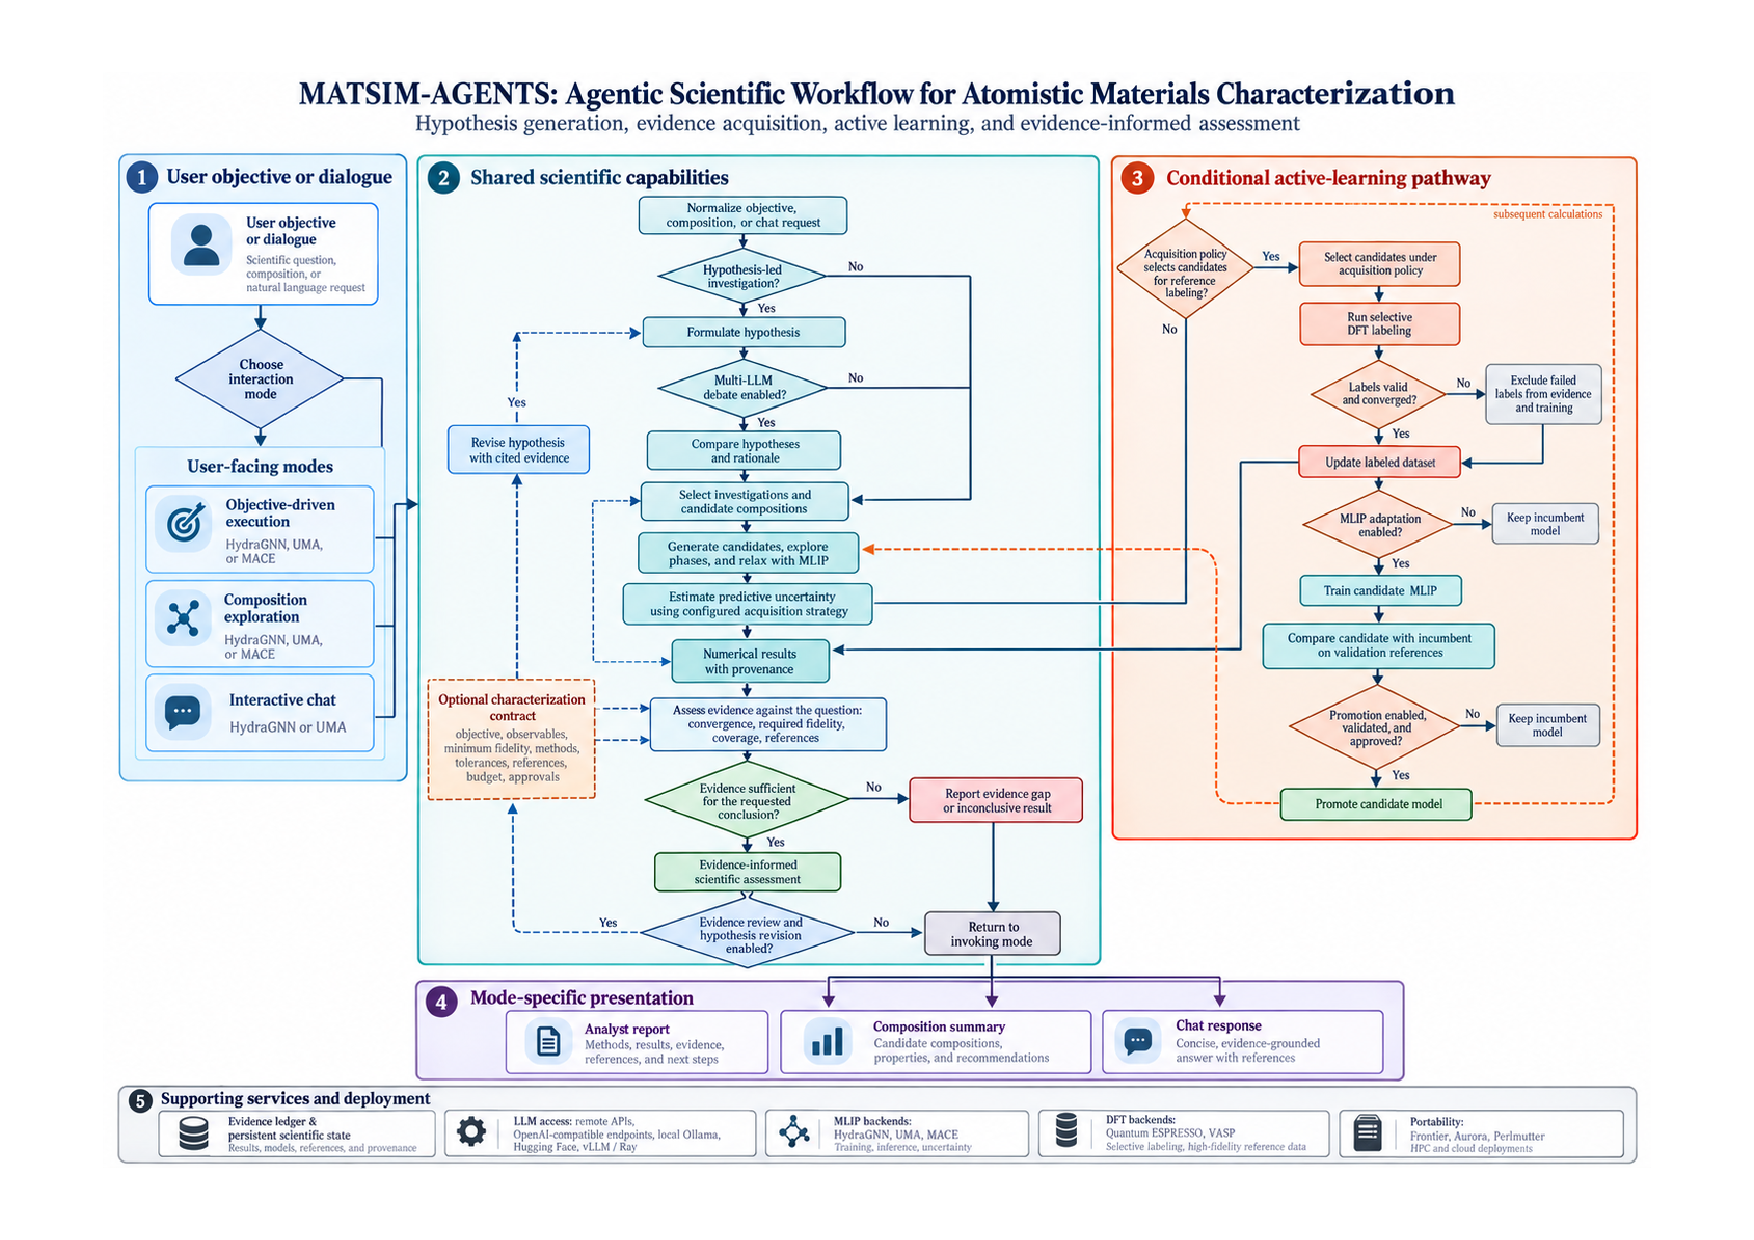
\includepdf[pages=1,fitpaper=true,pagecommand={\refstepcounter{figure}\label{fig:agentic_scientific_workflow}}]{figures/fig_agentic_workflow_A4_printable.pdf}

\subsubsection{Agent Graph and Nodes}
The agent graph is assembled with LangGraph~\cite{langgraph} and contains four
primary nodes:

\textbf{Planner.} A configurable \ac{LLM} selected through the provider interface turns the user objective into a typed list of \texttt{TaskSpec} items
(\texttt{relax}, \texttt{analyze}, \texttt{report}), using Pydantic schemas for
schema-validated \ac{JSON} parsing.

\textbf{Executor.} For each \texttt{relax} task the executor runs \ac{ASE}
\ac{FIRE}/\ac{BFGS} optimization with the selected \ac{MLIP} backend
(HydraGNN~\cite{hydragnn}, UMA~\cite{wood2025uma}, or
MACE-MP~\cite{batatia2022,batatia2023macemp}) as the force-and-energy evaluator,
appending the optimized structure, final energy, max force, and convergence flag
to the shared typed state.

\textbf{Validation Gate.} After relaxation, a configurable
\emph{post-relaxation gate} decides whether each optimized structure can proceed
to analysis or must be escalated to \ac{DFT}-driven \ac{AL}, based on the
relaxation outcome (convergence and residual forces) and the workflow's
exploration policy. On acceptance, it
passes control to the analyst; otherwise it triggers the \ac{AL} handoff, logging
the decision to a \ac{JSONL} audit file.

\textbf{Analyst.} The analyst node invokes the \ac{LLM} to generate a natural
language summary of the discovered structures, including energy rankings and
stability estimates.

\subsubsection{Entry Points and Task Complexity}
The nodes are exposed through three entry points of increasing scope. The
\emph{default linear graph} handles a single well-posed objective (e.g., ``relax
this structure and report its stability'') in one
planner$\rightarrow$executor$\rightarrow$gate$\rightarrow$analyst pass, the only
branch being escalate-or-summarize. The \emph{supervisor graph} adds a supervisor
over five nodes (prepare, explore, validate, optional \ac{AL}, summarize) that
iterates across a composition space and loops back into \ac{AL} when the gate
flags structures for escalation. The \emph{discovery chat} is an interactive
\ac{REPL} that adds automatic composition detection from free text, optional
multi-\ac{LLM} peer review, and slash commands (\texttt{/relax}, \texttt{/al},
\texttt{/clear}) for human-in-the-loop investigation.

\subsection{Candidate structures, atomistic characterization and scientific backends}

\paragraph{Structure provenance and acquisition.}
Composition proposals are converted to candidate configurations through the existing crystallographic-seed and symmetry-constrained generation interfaces, including AFLOW-based structure retrieval~\cite{curtarolo2012aflow} and PyXtal-based generation~\cite{fredericks2021pyxtal} where configured. \texttt{matsim\_agents.campaign.registry} maintains \texttt{StructureCandidateRecord} entries with candidate identifiers, composition, origin, prototype or space-group metadata, random seed, parent identifier and structure hashes. \texttt{CandidateEvaluationRecord} stores the chosen backend, checkpoint identity, convergence, energy, force and uncertainty or novelty descriptors. Candidate equivalence after relaxation is treated separately from equivalence of starting structures: relaxed-family clustering can prevent multiple structurally equivalent candidates from consuming the same acquisition budget. The registry also implements structure-content hashing and structure-averaged \ac{SOAP} descriptors~\cite{bartok2013soap} for structural novelty. Policy parameters for random, exploitation, exploration and adaptive acquisition are explicit and include exploration/exploitation quotas and limits on repeated selection from the same relaxed family. These choices are testable numerical selection policies, not proof that the selected configurations are novel phases.
The third layer performs the scientific computations by evaluating energies and forces with a
configuration-selected \ac{MLIP} backend and escalates flagged structures to
\ac{DFT} through the \ac{AL} and warm-start protocols. Three pretrained
potentials---HydraGNN~\cite{hydragnn,lupopasini2026exascalegfm},
UMA~\cite{wood2025uma}, and MACE-MP~\cite{batatia2022,batatia2023macemp}---sit
behind one calculator interface and are chosen by a single switch
(\texttt{MLIP\_BACKEND}) without alterations to the orchestration code.

\subsubsection{MLIP energies, forces and structural relaxation}

\paragraph{Computational interface and fidelity semantics.}
The shared calculator interface is implemented in the \texttt{matsim\_agents.backends.mlip} package and is consumed by \texttt{matsim\_agents.workflows.relaxation}. A numerical result records the structure used, optimized geometry, energies, residual forces, convergence and model identity. Cell relaxation requires stress information; the implementation preferentially uses backend-native stress and provides a finite-difference stress route when applicable. A relaxation terminated by its step limit is not treated as converged merely because its process exited normally. The characterization recipes enforce the difference between same-composition energy comparisons and thermodynamic stability against a set of competing phases. A convex-hull conclusion requires converged \ac{DFT} evidence and a method-compatible, sufficiently complete reference set. A surrogate hull is explicitly provisional and cannot alone certify first-principles thermodynamic stability.
Each backend implements the same calculator, acquisition, and labeling
interfaces; the workflow depends only on their shared contract---energy and force
evaluations that are orders of magnitude faster than direct \ac{DFT}. The default HydraGNN
\ac{GFM} is an exascale-pretrained multi-task graph model with wide chemical
coverage (architecture and pretraining detailed
in~\cite{lupopasini2026exascalegfm}); UMA~\cite{wood2025uma} and the MACE-MP
models~\cite{batatia2022,batatia2023macemp} are universal potentials used through
their released checkpoints. Any of the three can serve as a relaxation engine,
a warm-start pre-relaxer, or the initial model for \ac{AL}.

\subsubsection{Active learning and DFT evidence acquisition}

\paragraph{Acquisition, labeling and validation software.}
The acquisition loop resides in \texttt{matsim\_agents.active\_learning.loop}, with candidate production, uncertainty estimation, \ac{DFT} protocol definition and training delegated to corresponding modules in \texttt{matsim\_agents.active\_learning}. Ensemble disagreement and Monte Carlo dropout provide alternative uncertainty indicators~\cite{lakshminarayanan2017,gal2016,schran2020}; these scores motivate acquisition but are not interpreted as calibrated physical errors without validation. DFT label preparation preserves numerical protocol information, and the loop retains per-configuration provenance including candidate, seed structure, trajectory, time index, active-learning iteration and physical conditions. Labels from failed or unconverged calculations are tracked distinctly from admissible converged labels.

\paragraph{Independent adaptation assessment.}
\texttt{matsim\_agents.datasets.splits} constructs explicit training, validation and test partitions using frame, temporal-block, trajectory, structure-family, composition, condition, active-learning-iteration or declared group criteria. It writes content-addressed split manifests, hashes, membership lists and leakage diagnostics; missing metadata for a required grouping rule raises an error rather than invoking a silent frame-level fallback. The fine-tuning evaluator \texttt{matsim\_agents.active\_learning.finetune\_eval} requires such an evaluation configuration. HydraGNN, UMA and MACE can therefore be compared against identical partitions. Model selection or promotion is based on validation performance; the test partition is evaluated only after that decision is saved. \texttt{matsim\_agents.active\_learning.eval\_report} supports per-frame and per-group error summaries, paired differences, independent-group bootstrap intervals and comparisons across splits, training seeds and acquisition iterations. These tools establish a reproducible evaluation protocol; measured model improvements must still be obtained from the specified training campaigns.
When the validation gate escalates a structure, \textsc{matsim-agents} can execute a configurable number of active-learning iterations, following established uncertainty-guided and concurrent-learning approaches~\cite{smith2018,vandermause2020,vandermause2022,zhang2020dpgen,podryabinkin2017}. Figure~\ref{fig:acquisition_schematic} summarizes the numerical loop: short MLIP-driven molecular-dynamics trajectories generate off-equilibrium candidates; filtering and acquisition policies select snapshots; the selected structures are evaluated with a user-selected DFT solver; and converged labels are retained for optional backend-dependent MLIP adaptation. Each iteration records candidate counts, DFT convergence, timing, and other execution metadata in persistent state. Retraining and promotion are distinct decisions: adding DFT labels does not automatically authorize replacement of the deployed model. The detailed candidate-scoring methods and experimentally measured adaptation outcomes are provided in Section~\ref{sec:scientific_results}.

\begin{figure}[tb]
\centering
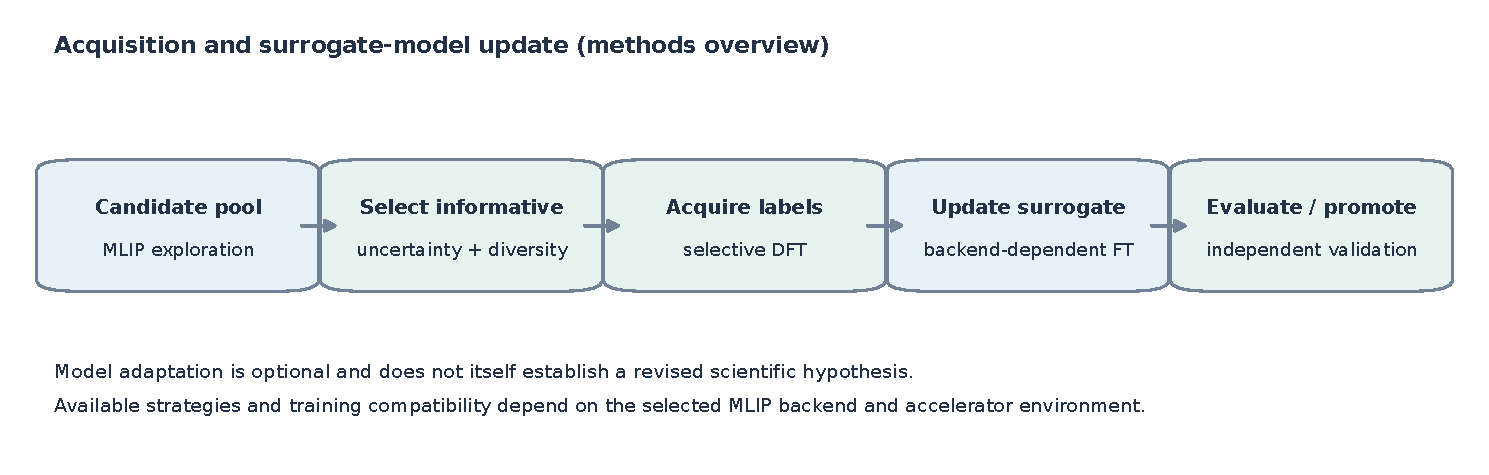
\includegraphics[width=\linewidth]{figures/fig_acquisition_vector.pdf}
\caption{\textbf{Numerical evidence acquisition and model adaptation.} This methods diagram concerns how atomistic evidence is collected and how a surrogate may subsequently be updated; it does not depict LLM hypothesis revision (Fig.~\ref{fig:evidence_revision}). Model promotion depends on independent validation, and the schematic does not establish calibrated uncertainty or superior acquisition efficiency.}
\label{fig:acquisition_schematic}
\end{figure}

The loop is backend-agnostic: the \ac{DFT} interface accepts a
\texttt{DFTJobSpec} and returns converged frames, so \ac{QE} (open source) and
\ac{VASP} (licensed, user-supplied source) are interchangeable from the workflow
perspective.

\subsubsection{MLIP-assisted DFT geometry optimization}
A separate warm-start benchmarking module pairs each \ac{MLIP} pre-relaxer
(HydraGNN~\cite{hydragnn} or UMA~\cite{wood2025uma}) with each \ac{DFT} solver
(\ac{QE} via \texttt{warmstart\_benchmark\_qe}, \ac{VASP} via
\texttt{warmstart\_benchmark\_vasp}) as a factorial ablation, so that any
warm-start benefit can be attributed to the potential, the solver, or their
interaction.

The benchmark pipeline, shared across all four configurations, proceeds as follows
for any input crystal structure: (i) an \ac{MLIP} \ac{FIRE} pre-relaxation to
$f_\text{max} = 0.01$\,eV/\AA\ (HydraGNN~\cite{hydragnn} or UMA~\cite{wood2025uma});
(ii) the selected \ac{DFT} solver from the \emph{original} coordinates (cold
start: \ac{QE} \texttt{vc-relax} or the equivalent \ac{VASP} ionic relaxation);
(iii) the same solver from the \emph{\ac{MLIP}-relaxed} coordinates (warm start);
and (iv) comparison of \ac{BFGS} step counts, per-step and total \ac{SCF}
iterations, final energies, and wall times. Identical \ac{DFT} input settings are
used for cold and warm runs to ensure a fair comparison.

% =============================================================================

\subsection{Evidence-informed hypothesis assessment, model adaptation and provenance}

\paragraph{Evidence ledger and claim validation.}
\texttt{matsim\_agents.execution.ledger} implements an append-only \ac{JSONL} ledger with three typed records: \texttt{EvidenceRecord} for measured or failed numerical calculations, \texttt{HypothesisRecord} for a claim and its revision history, and \texttt{DecisionRecord} for a consequential action and its cited evidence. Evidence records store a method signature, software and model identity, evidence level, convergence outcome, values and units, physical assumptions, completeness of phase references, parent evidence and hashes of input/output files. Content-derived identifiers make repeated identical records idempotent; a hash chain, checkpoint, file locking and artifact verification detect alteration or incomplete recording within the documented verification scope. The command \texttt{matsim-agents ledger verify} checks ledger integrity and, when requested, the recorded artifacts.

Validation rules require cited numerical evidence for supported or contradicted claims and for consequential decisions. Failed or unconverged calculations cannot support physical claims, and a thermodynamic-stability assessment cannot be established from MLIP-level evidence or an incomplete convex-hull reference set. The ledger therefore distinguishes an LLM-proposed judgment from an admissible scientific finding. Campaign and characterization workflows currently write ledger entries; standalone relaxation, phase exploration and independent active-learning invocations are not all covered by this ledger mechanism.
The structured scientific state links the initial claim and its falsifiable prediction to computed observables, method settings, evidence identifiers, uncertainty or limitations, claim assessments, subsequent revisions and proposed discriminating tests. Two different forms of revision occur within this workflow. The first concerns the scientific assessment: numerical observations may strengthen, contradict, or leave unresolved a claim about a material. The second concerns the numerical surrogate: selected \ac{DFT} calculations can provide labeled configurations for adapting a \ac{MLIP}. These updates serve different purposes and require different criteria for success. Lower prediction error for the MLIP does not itself establish a materials hypothesis, while a well-supported hypothesis may require no change to the surrogate. Model disagreement can motivate additional testing, but cannot independently certify material stability. The workflow records these decisions separately so that changes to a scientific conclusion can be traced to physical evidence rather than inferred from model-training progress.

\newexperiment{End-to-end hypothesis revision}{Run a complete hypothesis $\rightarrow$ simulation $\rightarrow$ evidence $\rightarrow$ LLM revision $\rightarrow$ new test sequence; release the structured state and compare the revised claims with independently checked numerical results. }

\subsection{Computational orchestration, backend interfaces and persistent execution}

\paragraph{Execution, recovery and resource records.}
Execution is divided among the orchestration layer, \texttt{matsim\_agents.execution} utilities, \ac{DFT} subprocess wrappers, and facility-specific launch scripts under \texttt{deployments/}. Typed launch placement represents nodes and the accelerator resources addressed on Frontier, Aurora and Perlmutter. Campaign and characterization state records allow completed steps to be reused when scientifically identical inputs and valid output artifacts are present. Run locks prevent two writers from concurrently changing the same execution state. \texttt{matsim\_agents.execution.recovery} classifies calculation, input, launch and infrastructure failures and applies bounded retry or restart policies; a retry is not treated as a successful numerical result until convergence criteria are met. The \ac{DFT} process layer also handles interrupted or timed-out process groups so an abandoned subprocess does not continue consuming resources after its parent workflow has stopped.

The \texttt{CostRecord} attached to numerical evidence distinguishes LLM tokens and inference time, MLIP calculations, DFT attempts, adaptation effort and failed jobs. When resource placement is resolved it additionally reports allocated node-hours and accelerator-device or physical-GPU hours, retaining the architecture-specific device distinctions. For fair comparisons of scientific strategies, accumulated costs must include unsuccessful attempts and recovered calculations as well as successful evidence. Backend capability checks, resumability and process cleanup improve operational reproducibility; their quantitative effects require separately reported tests. The practical separation of Python, accelerator and first-principles runtime environments, including platform launch procedures, is documented in Appendix~\ref{sec:hpc:platform_design} and Appendix~\ref{sec:hpc:platform_deployment}. Detailed restart and throughput checks belong to Appendix~\ref{sec:results_reliability}; these operational tests do not substitute for scientific characterization accuracy.
The LLM, MLIP and DFT backend abstractions serve different purposes. LLM substitution tests the robustness of hypothesis representation and reasoning; MLIP substitution tests surrogate-dependent numerical behavior and cost; DFT substitution tests functional workflow interchangeability under a documented method comparison. Backend-independent orchestration must preserve units, physical semantics, calculation settings and provenance. Backend selection must not silently change the scientific question.

The common-interface scientific comparison and the limitations of backend interchangeability are developed further in Appendix~\ref{sec:results_interoperability}; method-matched reference calculations remain necessary when physical observables are compared across DFT codes.

\newexperiment{Three-layer backend interoperability}{Exercise at least two LLM configurations, two MLIPs and both VASP/QE through common typed interfaces on matched tasks. Document the exact extent of full-loop execution, configuration differences, failure modes and comparability of physical observables.}


\subsubsection{Architecture-independent execution across leadership computing facilities}
\label{sec:methods:portability}
The same characterization contract, scientific-task graph, evidence requirements and scientific decision policy are defined independently of the computer on which calculations execute. Platform-specific resource descriptions and launcher scripts mediate access to the numerical engines rather than changing the workflow's scientific semantics. The implementation separates (i) typed backend capability information in \texttt{matsim\_agents.execution.capabilities}, (ii) job placement and process management in \texttt{matsim\_agents.execution.placement} and \texttt{matsim\_agents.backends.dft.process}, and (iii) facility-specific environment setup and launch scripts under \texttt{deployments/frontier/}, \texttt{deployments/aurora/} and \texttt{deployments/perlmutter/}. The \texttt{matsim-agents capabilities check} and \texttt{capabilities matrix} commands distinguish declared backend support from dependencies available at runtime. Launcher scripts configure the local compiler, accelerator, Python and message-passing environments, while backend adapters provide a common scientific interface for relaxation and first-principles calculations.

Portability is assessed at three distinct levels: the availability of a configured backend, successful execution of equivalent scientific tasks, and agreement of the resulting scientifically relevant observables. These are not interchangeable claims. A successful backend installation or scripted test does not establish that an entire characterization campaign has run on every facility. Moreover, reproducible scientific conclusions do not imply identical trajectories, operation counts or timings across different accelerator and numerical-library implementations. Calculation records therefore retain model and software versions, numerical settings, execution outcomes and resource placement. This distinction is tested explicitly in Section~\ref{sec:results:crossplatform}. Facility-specific environment modules, accelerator runtimes and DFT launcher requirements are documented in Appendix~\ref{sec:hpc}, while the corresponding execution and restart performance investigations are described in Appendix~\ref{sec:results_reliability}.


\subsection{Distinguishing hypothesis revision from surrogate-model adaptation}
The numerical and scientific feedback processes are related but serve different objectives. First-principles energies and forces collected for selected configurations can be incorporated into an MLIP training set, followed by model selection using validation data that are independent of the final test set. This adaptation modifies the approximation used for subsequent atomistic calculations. Separately, numerical observations from converged calculations can be supplied to the scientific reasoning layer to reconsider a hypothesis regarding a candidate composition or configuration. Improved surrogate accuracy does not itself establish the validity of a materials hypothesis; the assessment depends on the physical quantities and reference calculations required by the particular claim. The campaign state preserves the distinction between updated model parameters, computed observables and scientific assessments.
\section{Test cases and numerical setup}
\label{sec:methodology}

\subsection{Allocation-efficient experimental design and staged qualification}
\label{sec:setup:cost_staging}
The numerical program comprises four principal experiments and one proposed supplementary assessment: (E1a) workflow-aligned scientific hypothesis formulation, (E1b) a proposed separate cross-domain generalization assessment, (E2) fixed-evidence characterization and hypothesis assessment, (E3) adaptive characterization with selective reference acquisition and optional surrogate adaptation, and (E4) execution portability across three supercomputing architectures. E1b remains subject to independent scientific review and is not part of E1a held-out evaluation. Experiments are ordered by the additional numerical evidence they require rather than by available backend combinations. Measured results, archived evidence replay, and unperformed experiments are distinguished throughout Section~\ref{sec:numerical_results}.

\paragraph{Reusing reference calculations.}
Before allocating new computational resources, existing DFT structures, energies, forces, convergence histories and numerical settings are reconciled against an experiment manifest. An archived result can be reused only when its structure, numerical method, physical assumptions and provenance satisfy the corresponding scientific contract. For evidence-replay comparisons, both assessment policies receive the same frozen evidence; replay cannot incur new DFT calculations. For adaptive policy replay, the candidate pool may be fully labeled for evaluation purposes, but unselected reference values must remain hidden from both acquisition policies. A content- and method-aware cache avoids repeating identical physical calculations requested by different policies, while each policy's hypothetical expenditure is accounted for independently.

\paragraph{Staged execution and stopping criteria.}
The experimental sequence is: (0) audit reusable data, checkpoints and logs across all six material systems; (1) evaluate E1 hypotheses and E2 fixed-evidence assessments with class-stratified objectives and reference packets; (2) qualify MLIP, DFT and scheduler pathways using bounded workloads; (3) evaluate zero-shot HydraGNN, UMA and MACE predictions for every supported material--model combination with independent validation criteria; and (4) apply the same budget-controlled acquisition, scientific assessment and conditional adaptation protocol to each supported combination that fails the prespecified validation thresholds. Preliminary workloads calibrate execution and cost but do not determine which material classes are eligible for E3. Additional DFT execution is authorized only for unresolved numerical requirements after checking compatible stored evidence. The E4 cross-facility benchmark is a bounded qualification rather than a repetition of all materials and model combinations. Before each stage, the experiment manifest specifies the scientific question, dataset version, backend, random seeds, maximum resource expenditure, expected artifacts, assessment rules, and conditions for continuation. Pilot failure modes, reference inconsistency, and insufficient independent samples are addressed before expansion; termination criteria are prespecified rather than selected based on whether a method appears favorable.

\paragraph{Cost and fairness.}
The primary live C-versus-D comparison fixes an identical ceiling on attempted DFT calculations or on a prespecified, facility-specific DFT resource budget. All outcomes, including failed attempts and retries, are charged to the requesting policy. Total cost is reported separately for LLM tokens and inference time, MLIP inference, DFT node-hours, model training, and orchestration. Accelerator-hours and node-hours from different machines are not summed as if their hardware or charging rates were interchangeable. Scientific resolution is plotted against cumulative budget, and justified inconclusiveness is scored separately from successful supported or contradicted conclusions.

\begin{table}[htbp]
\centering\small
\caption{Cost-aware progression of the principal numerical studies. The stages are experimental design commitments, not reported results.}
\label{tab:allocation_priority}
\begin{tabularx}{\linewidth}{@{}p{0.10\linewidth}p{0.29\linewidth}p{0.21\linewidth}X@{}}
\toprule
Study & Comparison & Preferred evidence source & New allocation trigger \\
\midrule
E1a & Local/remote individual reasoning and structured-collaboration ablations & Expert-reviewed six-material, workflow-aligned question bank and model inference & No DFT required; validate selected hypotheses only downstream \\
E1b (proposed) & Separate supplementary cross-domain generalization assessment & Proposed 12-question bank; independent review pending & No E1b inference authorized; maintain separate questions, outputs and accounting \\
E2 & C versus D on identical evidence & Archived DFT and known-answer replay & Fill only verifiable gaps in the reference library \\
E3 & C versus D adaptive acquisition and revision & Cached candidate pool, followed by bounded live runs & Pilot establishes fair budgets, valid labels and useful decision variation \\
E4 & Shared characterization across three facilities & Small, fixed qualification workload & Execute once per required facility/backend combination \\
\bottomrule
\end{tabularx}
\end{table}
The evaluation must distinguish three different claims: (a) scientific tools generate usable numerical evidence; (b) numerical evidence improves the reliability of MLIPs and task-dependent decision policies; and (c) returning this evidence to an LLM improves its scientific hypotheses or next-test proposals. Measurements of (a) or (b) alone cannot establish (c).

\subsection{MLIP datasets, independent partitions and model evaluation}
For each scientific objective, define a split unit corresponding to the intended generalization claim (independent MD trajectory, starting structure, composition, physical condition, or active-learning campaign). Model weights and reference corrections are fitted on training data; model selection, calibration and promotion decisions use validation data; the held-out test is untouched until evaluation. Random frame splits remain useful for within-distribution interpolation but should not be described as independent-trajectory or composition transfer.
\newexperiment{Statistically independent model comparisons}{Reconstruct dataset lineage; create independent training/validation/test groups; rerun MLIP fine-tuning with multiple seeds; report paired test errors and confidence intervals across independent groups. In particular, never select a best backend using the final test partition.}

The repository also contains a Codabench-compatible multi-task benchmark (\texttt{benchmarks/codabench/}) for comparing interatomic-potential predictions under common reference conventions. Its five tasks cover formation energy per atom, atomic forces, relaxed structure, MLIP-assisted DFT relaxation, and energy ranking within fixed-composition groups. These numerical-model assessments are separate from the comparison of LLM-guided and deterministic scientific decision policies. The benchmark definitions, scoring metrics and public/private partition protocol are specified in Appendix~\ref{sec:appendix:codabench}. Compatibility with the Codabench submission and scoring format does not, by itself, establish that a public competition or externally validated leaderboard has been operated.

\subsection{LLM configurations and controlled comparisons}

\paragraph{Executable reasoning and known-answer test suites.}
Two complementary suites are available under \texttt{benchmarks/}. The \texttt{agent\_eval} cases provide fixed claim/evidence inputs for paired reasoning-policy comparisons; these synthetic or representative records must not be described as independent DFT observations. The \texttt{known\_answers} suite contains five Si/SiC characterization tasks whose expected properties or admissible outcomes are specified before execution: silicon lattice constant, diamond-versus-$\beta$-tin energy ranking, two silicon-carbide hull cases, and correctly inconclusive reporting of a step-limited relaxation. Its replay tier checks generated Quantum ESPRESSO input against stored input and returns the corresponding recorded output; its live tier invokes the solver. The initial five cases provide a reproducibility and protocol-verification baseline, not a statistically comprehensive materials-science evaluation. The publication-level experiment should extend these cases and compare LLM and deterministic strategies on identical evidence, scientific questions and resource budgets.
For each hypothesis, prespecify testable predictions, a reference evaluation protocol and a rubric for interpreting evidence. The principal comparison uses two capability-matched assessment policies: (C) LLM-guided interpretation and calculation selection and (D) deterministic rule-based interpretation and adaptive calculation selection. Both use the same characterization contracts, evidence ledger, numerical backends, admissibility checks, scientific inputs and resource budgets. A fixed-evidence evaluation isolates interpretation from acquisition, while live characterization permits the policies to request different calculations within the same budget. Separately, Section~\ref{sec:results_llm} compares single-LLM and multi-LLM hypothesis formulation without introducing an intentionally unvalidated characterization arm. Score conclusion correctness, appropriately unresolved outcomes, unsupported claims, proposed follow-up test informativeness and the total cost per independently validated result.
\newexperiment{LLM-guided versus rule-based scientific assessment}{Conduct replicated controlled comparisons of policies C and D using identical initial problem statements, admissibility checks and matched numerical validation. Archive prompts, reasoning outputs, tool traces, physical results and blinded expert or rule-based scoring. Any multi-LLM debate variation is evaluated within policy C, not as a separate less-validated comparison arm.}

\subsection{Uncertainty criteria and active-learning controls}
Decisions about polymorph energies, relaxation or dynamical stability require task-specific observables; a single global force MAE does not validate all decisions. Uncertainty from ensembles or MC dropout requires empirical calibration against independent DFT reference data.
\newexperiment{Task-specific decision gates}{Specify thresholds and comparison operators before test evaluation. Report false-acceptance rate, escalation rate, scientific decision error and DFT expenditure against a fixed-rule baseline. Evaluate the decision policy using unrounded source metrics.}

\subsection{Dataset provenance and computational resources}
Identify generated candidates, screened frames, converged DFT calculations, exclusions, deduplication, and configurations used in every train/validation/test partition. Archive calculation methods, random seeds, run identifiers, model checkpoints, software revisions and LLM inference cost. Appendix~\ref{sec:results_synthesis} details the integrated resource-accounting considerations, and Appendix~\ref{sec:results_reliability} records supporting execution-throughput and restart measurements; the main comparison must nevertheless report its total costs and failures.
\newexperiment{Dataset reconciliation and full cost accounting}{Report the complete flow from converged DFT outputs to training configurations; include separate LLM service latency, GPU time, token counts and failed computation costs. Publish a runnable provenance-to-figure reproduction script.}
\subsection{Materials systems, structures and first-principles settings}
\label{sec:results:setup}
The atomistic calculations were executed on NERSC Perlmutter. The systematic evaluation considers six materials systems: LiFePO$_4$, the Cantor FCC alloy, NbTaVHfZrTi BCC alloy, phosphorene, Zn(HCOO)$_2$ metal--organic framework, and the Nb--Ta--O composition space. The previously reported VASP labeling campaign covers the first five systems; Nb--Ta--O follows a separate, method-specific Quantum ESPRESSO protocol and is not included in that campaign's numerical totals. The VASP settings for the five previously reported systems are summarized below.

The warm-start and fine-tuning studies use a single compute node
(4$\times$ NVIDIA A100 80\,GB), whereas the end-to-end campaigns and
strong-scaling study use one to eight such nodes, as specified below. The five
previously reported VASP end-to-end test systems span diverse chemistries and dimensionalities:
LiFePO\textsubscript{4} olivine (3D battery cathode), NbTaVHfZrTi \ac{BCC} and
CrMnFeCoNi Cantor FCC \acsp{HEA} (3D refractory and structural alloys),
phosphorene (2D semiconductor), and the Zn(HCOO)\textsubscript{2} \ac{MOF} (3D
porous framework).

Each \ac{AL} iteration follows the scientific-computation stages in
Fig.~\ref{fig:architecture}. Seed structures are propagated by short Langevin
\ac{MD} trajectories (400 steps, 2\,fs, 1000\,K) under the selected \ac{MLIP}
force engine; snapshots are subsampled every 15 steps and screened by force and
displacement thresholds; surviving candidates are down-selected under a
per-iteration budget with a composition-diversity filter; selected frames are
labeled by concurrent single-point \ac{VASP} calculations; and converged frames
are appended to the growing training set. State is checkpointed after each
iteration so a campaign can resume after a wall-time boundary.

The single-point \ac{DFT} settings used to label every frame are summarized in
Table~\ref{tab:dft}. All systems use the same Perdew--Burke--Ernzerhof (PBE)
generalized-gradient exchange--correlation functional with projector
augmented-wave (PAW) potentials, providing a consistent reference across
chemistries; per-case choices vary only in spin treatment, smearing, and k-point
density. The magnetic $3d$ systems (LiFePO\textsubscript{4} and the CrMnFeCoNi
Cantor alloy) are computed with spin polarization (\texttt{ISPIN}$=2$); no
Hubbard $+U$ correction is applied to any system, so the
LiFePO\textsubscript{4} reference uses spin-polarized \ac{GGA} without a $+U$
correction. The five VASP datasets use the same functional because the
focus of this study is the orchestration workflow and the surrogate's ability
to reproduce a common \ac{DFT} reference rather than the absolute
materials-specific accuracy of any single system. More specialized \ac{DFT}
settings could improve the fidelity of individual reference datasets, but such
materials-specific treatment is outside the scope of the present workflow
evaluation.

\begin{table}[tb]
\centering
\caption{Per-case single-point \acs{VASP}/PAW settings. Shared across all cases:
PBE (\ac{GGA}) functional, \texttt{ENCUT}$=520$\,eV, \texttt{EDIFF}$=10^{-6}$\,eV,
$\Gamma$-centred k-meshes, \texttt{NSW}$=0$, and no Hubbard $+U$.}
\label{tab:dft}
\footnotesize
\setlength{\tabcolsep}{4pt}
\resizebox{\columnwidth}{!}{%
\begin{tabular}{lccc}
\toprule
System & Spin (\texttt{ISPIN}) & Smearing ($\sigma$/eV) & \texttt{KSPACING} (\AA$^{-1}$)\\
\midrule
LiFePO\textsubscript{4} olivine     & polarized (2)   & Gaussian (0.05) & 0.30 \\
CrMnFeCoNi Cantor FCC \acs{HEA}     & polarized (2)   & MP-1 (0.20)     & 0.22 \\
NbTaVHfZrTi BCC \acs{HEA}           & unpolarized (1) & MP-1 (0.20)     & 0.25 \\
Phosphorene (black-P)               & unpolarized (1) & Gaussian (0.05) & 0.25 \\
Zn(HCOO)\textsubscript{2} \acs{MOF} & unpolarized (1) & Gaussian (0.05) & 0.30 \\
\bottomrule
\end{tabular}%
}
\end{table}


\subsection{Cross-platform scientific workload and computing environments}
\label{sec:setup:portability}
The targeted systems represent three accelerator ecosystems: OLCF Frontier (AMD Instinct MI250X; ROCm/HIP), ALCF Aurora (Intel Data Center GPU Max; oneAPI/Intel GPU stack) and NERSC Perlmutter (NVIDIA A100; CUDA). The physical allocation unit and logical accelerator device differ across the platforms; Frontier has eight GPU compute dies per node, Aurora has twelve GPU tiles per node, and Perlmutter GPU nodes have four A100 GPUs. Consequently, accelerator-device counts, physical GPU counts, GPU-hours and node-hours must be reported with explicit definitions rather than interpreted as directly equivalent across systems.

A controlled portability qualification should use the same characterization contract and initial structure on all three platforms, with a common observable set, numerical tolerances and scientific decision rules. The existing \texttt{benchmarks/portability/} harness supplies a common scientific configuration, facility overlays, task runners and validation tools. For every platform and computational component, record the repository commit, numerical backend/model and checkpoint, software versions, launcher configuration, node and accelerator allocation, outcome, convergence status and the hashes of generated scientific artifacts. Backend availability, successful numerical execution and full-workflow completion should be tabulated separately. Where different numerical engines or model implementations are necessary, document these substitutions and interpret numerical differences as a combined method/platform effect rather than pure architectural variation.

\newexperiment{Matched three-facility qualification}{Execute the same representative characterization contract on Frontier, Aurora and Perlmutter with verified MLIP relaxation, DFT verification, evidence assessment and final report wherever supported. Publish per-stage success/failure, energy and force tolerances, structural agreement, convergence, walltime and resource allocation. Do not mark an unavailable backend as a successful portability test; do not infer full-workflow validation from a launcher smoke test.}


\subsection{Reference characterization tasks, baselines and evaluation metrics}
\label{sec:results_protocol}
\noindent\textbf{Benchmark unit.} Each task is specified by a material/configuration, an explicit characterization question, permitted computational methods, a precommitted reference protocol, numerical tolerances, a task-dependent stopping rule, and an identical computational budget across arms. The intended task families span structural convergence, fixed-composition energy ordering, phase-stability evidence, surrogate reliability, and incomplete or contradictory calculations. The reference assessment distinguishes a physically justified conclusion from a justified decision that the evidence is insufficient.

\noindent\textbf{Two complementary test regimes.} (i) \emph{Evidence replay}: a provisional target of 30--50 independently reviewed cases with frozen numerical results and provenance, used to test scientific interpretation without charging the agent for new numerical simulation; (ii) \emph{live characterization}: a provisional target of 8--12 diverse cases requiring actual numerical tool selection, evidence acquisition, and stopping decisions. These targets are revised after a pilot assessment of task variability and statistical precision, not fixed as evidence of study power. Correlated atomistic configurations do not constitute independent characterization cases; scientific reference outcomes and final evaluation cases are specified independently of prompt and policy development.

\begin{table}[htbp]
\centering\small
\caption{Primary capability-matched characterization policies. Both policies use identical scientific contracts, evidence-admissibility rules, numerical backends, candidate pools, uncertainty inputs and computational budgets.}
\label{tab:characterization_arms}
\begin{tabularx}{\linewidth}{@{}p{0.09\linewidth}p{0.40\linewidth}X@{}}
\toprule
Policy & Scientific assessment and investigation & Common safeguards and distinguishing mechanism \\
\midrule
C & MATSIM-AGENTS: LLM-guided hypothesis assessment and selection of follow-up calculations & Deterministic characterization contracts and ledger validation; the LLM proposes scientific interpretations and investigation decisions \\
D & Non-LLM adaptive workflow: rule-based hypothesis assessment and algorithmic selection of follow-up calculations & Identical contracts and ledger validation; predefined numerical rules and acquisition policies replace LLM reasoning \\
\bottomrule
\end{tabularx}
\end{table}

\noindent\textbf{Primary endpoint.} The principal outcome is the fraction of scientifically resolved tasks as a function of cumulative numerical and language-model inference cost. Supported conclusions and justified inconclusiveness are distinguished rather than pooled into a single favorable score. Secondary outcomes include unsupported-claim rate, missed-resolution rate, appropriateness of the next calculation, DFT labeling expenditure (including failed runs), human intervention, and numerical protocol violations. Statistical comparisons are paired at the level of independently defined tasks; repeated stochastic evaluations characterize variability within tasks. Computational expenditure includes unsuccessful calculations and, where relevant, model adaptation. A fixed offline labeled pool can be used for acquisition replay only if unselected labels remain hidden from each policy.

\newexperiment{Integrated characterization benchmark and matched baselines}{Construct and independently review the common evidence-replay and live-task collections. Preregister material selection, task inclusion, numerical tolerances, gold-standard conclusions, supported abstention reasons, stopping conditions, computational budgets and the primary endpoint. Evaluate C and D on identical frozen-evidence cases and on matched live characterization tasks. Use the same evidence-validation rules in both policies, and report any decisions rejected by those rules separately from the policies' initial proposals. Assess single- versus multi-LLM reasoning separately in Section~\ref{sec:results_llm}. Report paired, task-level success-versus-budget curves; separate successful characterization from justified inconclusiveness, failure and unsupported claims. At least one task/material should be independent of the development cases.}

\section{Numerical results}
\label{sec:numerical_results}
The numerical investigation follows the progression from scientific hypothesis formulation to structure-based assessment and finally to active acquisition of higher-fidelity evidence. The same material hypotheses and candidate stoichiometries are followed across these stages where the available records permit direct comparison. Numerical evidence supports conclusions only within the scope of its physical approximations; missing evaluations are identified in red rather than treated as measured outcomes. Backend-sensitivity comparisons are specified in Appendix~\ref{sec:results_interoperability}, with scaling, recovery, and performance analyses in Appendix~\ref{sec:results_reliability}.

\subsection{E1a: Workflow-Aligned Scientific Hypothesis Generation Across Local and Remote Frontier LLMs}
\label{sec:results_llm}
E1 evaluates local and remotely served LLM configurations for scientific hypothesis generation and structured collaboration. It does not presume that either deployment group is scientifically superior, that local and remote models are capability matched, or that observed group differences are caused by hosting location. Its scientific objective bank spans six systems: LiFePO$_4$, the Cantor FCC alloy, the NbTaVHfZrTi BCC alloy, phosphorene, Zn(HCOO)$_2$ MOF, and Nb--Ta--O. The latter probes composition-dependent oxide formation, competing phases, and the limitations of an incompletely sampled reference hull. Hypotheses and proposed numerical tests are scored independently; agreement among language models is not treated as physical evidence.

\paragraph{Research questions.}
E1 addresses three empirical questions. \textbf{RQ1 (individual scientific reasoning):} How do individually qualified, locally hosted open-weight models and remotely accessible frontier LLMs perform on scientific correctness, physical reasoning, falsifiability and evidence awareness? \textbf{RQ2 (structured debate):} Does complementary multi-LLM debate improve response quality relative to individual models, deterministic aggregation and additional independent reasoning, and does any measured benefit differ between panels composed of local and remote models? \textbf{RQ3 (quality and efficiency):} What tradeoffs are observed in scientific performance, reproducibility, confidentiality controls, accelerator and infrastructure resources, operational overhead, inference latency and expenditure? These questions remain open until the planned evaluation is completed.

\paragraph{Preliminary ablation: question design and individual-model scientific qualification.}
Before testing the effects of debate, operationally eligible local and remote LLM configurations are assessed independently using the same development question bank spanning the six material systems. Eligibility requires a pinned model identity or provider model/version record, documented licensing and institutional authorization, reproducible serving settings, and complete, parseable responses; serving success alone is not evidence of scientific competence. Models are characterized by deployment group for descriptive and stratified analysis, while model-specific capability, training, context and serving differences are retained as potential confounders rather than attributed to hosting. The bank has three recurring types of scientific reasoning task: (A) \emph{controlled comparison}, requiring models to distinguish competing mechanisms and specify discriminating tests; (B) \emph{evidence audit and falsification}, requiring them to identify supported conclusions, missing information, unjustified extrapolations, and outcomes that could reverse a conclusion; and (C) \emph{open-ended hypothesis generation}, requiring multiple physically plausible, nonredundant hypotheses with testable predictions and feasible numerical investigations. The third category tests the ability to formulate hypotheses rather than merely critique supplied claims. Evidence-audit questions qualify individual reasoning here; they do not replace E2's controlled, workflow-level fixed-evidence assessment.

The preferred feasibility bank comprises 36 independently authored questions: 18 development and 18 held-out questions, with one question of each type per material in each partition. A 24-question alternative (two development and two held-out items per material) is reserved for a lower-cost feasibility pilot if resource estimates require it; a one-question-per-partition smoke test supports only software qualification. Development and held-out items must involve distinct scientific situations rather than near-duplicate prompts. Each question has a frozen expert-reviewed packet specifying the scientific objective, supplied verified or explicitly hypothetical evidence, relevant assumptions, defensible reasoning paths, known limitations, unacceptable overclaims, and scoring anchors. In open-ended tasks no unique proposed hypothesis is assumed to be the sole correct response. All candidate models receive the same question and response contract: conclusion or hypotheses, physical mechanisms, assumptions, supporting and missing evidence, falsifiable predictions, discriminating tests, and interpretations of possible test outcomes. E1 does not ordinarily require new DFT calculations.

Blinded scientific reviewers score individual responses for scientific correctness, physical reasoning, falsifiability and informativeness of tests, evidence awareness, and feasibility of the proposed investigation. Provisional rubric weights of 30\%, 20\%, 20\%, 20\%, and 10\%, respectively, and anchored eligibility thresholds are frozen before candidate scores are inspected; independent review and adjudication of substantive disagreement are planned. Scores are summarized by task category and material, with material-level macro-averages, and response-format failures are reported separately from errors of physical understanding. Models failing the prespecified correctness or evidence-awareness threshold cannot enter the selected panel merely because their proposals differ from those of other models.

\paragraph{Development-set panel selection: competence, complementarity and cost.}
Among individually qualified models, candidate triples are compared for the scientific complementarity of their \emph{defensible} mechanisms, assumptions, recognized evidence gaps, predictions and proposed falsification tests, as well as their overlap in scientific errors. Textual dissimilarity, arbitrary disagreement, developer diversity and parameter count are not proxies for complementary scientific insight. Selection jointly considers individual competence, domain-relevant complementarity, computational cost and reproducible availability. A ranked shortlist and rationale are recorded; the final three-model panel, prompts, model revisions, grading rubric, aggregation rule and budget controls are frozen before held-out questions are opened. This qualification and selection stage does not itself establish that debate improves reasoning.

\paragraph{Held-out ablation: peer interaction versus additional inference.}
The qualified configurations and, where sufficient qualified participants exist, deployment-stratified panels are evaluated on identical held-out questions using (i) each constituent model acting alone, including the strongest individually qualified model overall and the strongest in each deployment group as prespecified baselines; (ii) a deterministic combination of three independent, noncommunicating model responses; (iii) an independent reasoning or self-revision condition using additional inference without exposure to peer arguments; and (iv) a structured two-round three-model debate with equal authority, rotated speaking order and independent final verdicts. Local-only and remote-only debate comparisons are made only when panel eligibility and sample size permit; mixed panels may additionally assess cross-deployment complementarity. Where standalone and independent-ensemble prompts and settings coincide, their responses are reused rather than regenerated or counted as independent observations. The additional-reasoning control is budget-matched to debate as closely as possible using measured calls and tokens, allowing the effect of peer criticism to be distinguished from additional inference expenditure. No unmeasured LLM synthesizer is inserted into the independent ensemble.

Primary scientific comparisons assess correctness, defensible and falsifiable hypotheses, appropriate recognition of missing evidence, useful discriminating tests and unjustified confidence; analysis of debate transcripts also tracks corrected errors, overlooked mechanisms, newly introduced mistakes and unsupported consensus. Evaluation is paired by independent question, stratified by material, task type and deployment group where estimable, and reports actual prompt/completion/reasoning tokens where available, number of calls, latency, serving overhead, API expenditure, facility-specific node/accelerator allocation and other attributable local serving costs. Confidentiality is evaluated as a documented data-governance and deployment-control profile, not inferred from a local endpoint. Repeated generations quantify within-question variation but are not counted as additional independent scientific tasks. Neither the 24- nor 36-question feasibility designs establishes broad generalization or a statistically reliable winning strategy; the observed differences are exploratory and motivate a separately powered follow-up if needed.

\newexperiment{E1a: Workflow-Aligned Scientific Hypothesis Generation Across Local and Remote Frontier LLMs}{Prepare expert-reviewed development and held-out question banks spanning all six materials and the three question types, preferably 18 questions per partition. Qualify authorized local and remote LLM configurations individually using blinded anchored scientific scores; enforce prespecified correctness and evidence-awareness thresholds and record model/version, license, deployment, governance controls, reproducibility settings and cost. Freeze qualified model sets and panel-selection rules using development data only. On held-out items compare individually qualified models, the strongest individual baseline, deterministic independent aggregation, budget-matched independent reasoning/self-revision, and equal-participation two-round debate with independent verdicts. Where panel size permits, compare local-only, remote-only and mixed panels on the same questions. Report outcomes by material, task and deployment group, alongside uncertainty, expert disagreement, scientific revisions, unsupported claims, falsifiability, latency, service expenditure, local compute and operational costs. Interpret this feasibility evaluation as exploratory: model capability and deployment are confounded, and neither group differences nor consensus establish a causal hosting effect or physical correctness.}

\textcolor{red!80!black}{\emph{Results pending:} numerical comparisons and representative hypothesis/debate trajectories for the material systems introduced in Section~3.}

\subsection{E1b: Proposed Supplementary Cross-Domain Generalization Assessment}
\label{sec:results_e1b}
E1b is proposed as a separate 12-question supplementary assessment of transfer beyond the material-specific contexts used for E1a. Its initial concept map covers charged point defects and chemical potentials, diffusion barriers and transport rates, surface adsorption and catalytic reaction barriers, harmonic phonons and finite-temperature stability, electrochemical voltage and reaction kinetics, and configurational entropy in alloys. Each proposed item uses explicitly hypothetical qualitative evidence, with no asserted measurement or numerical reference value; any future evidence-bearing packet requires independently verified source and method provenance. Domain-specific scoring anchors refine the shared scientific rubric around distinctions such as defect formation versus charge compensation, migration barriers versus transport rates, adsorption energies versus reaction barriers, harmonic dynamical stability versus finite-temperature stability, equilibrium voltage versus kinetics, and ordered-cell energy versus configurational free energy.

E1b is not an extension of the E1a held-out set. Its question bank, review, hashes, output records, and any future accounting are maintained separately. Freeze the E1a prompts, panel, and conditions before E1b exposure; E1b responses must not be used to revise those choices and then be described as an independent generalization test. The 12-question target is an initial proposal subject to independent scientific review, not a powered comparison or a frozen benchmark. No E1b inference or results are reported. E1a addresses workflow-aligned hypothesis generation; E2 tests fixed-evidence interpretation; E3 tests adaptive numerical evidence acquisition and conditional model adaptation; and E4 assesses computational portability. These complementary experiments evaluate distinct stages of the evidence-to-investigation process, not interchangeable proxies for general reasoning.

\subsection{Fixed-evidence characterization and evidence-informed hypothesis assessment}

\label{sec:results_phase}
\paragraph{Experiment E2: capability-matched fixed-evidence characterization.}
Under the fixed-evidence protocol, an independently adjudicated set of scientific questions and evidence packets represents each of the six material systems, subject to sufficient verified reference data. The LLM-guided policy (C) and the deterministic policy (D) receive the same converged and unconverged numerical results, method information, reference completeness and provenance. Both must satisfy identical \texttt{CharacterizationContract} requirements and the same evidence-ledger validation rules before a conclusion is accepted. The LLM proposes an interpretation and any additional tests; the non-LLM policy applies predefined numerical and scientific decision rules. This controls for the effect of evidence access and admissibility enforcement while testing the incremental scientific interpretation provided by language models. Raw proposed conclusions and final validated conclusions are reported separately so that rejection by the shared safeguard is not misattributed to reasoning quality. An unconstrained LLM without evidence checks is not included as a primary scientific comparator. Every archived DFT result is generated or retrieved once, with the same evidence packet supplied to both policies; the comparison incurs no additional DFT allocation when that packet is complete.
For the Nb--Ta--O evidence packets, distinguish rankings within a fixed composition from claims of stability across compositions: the latter require converged calculations and a sufficiently complete, internally compatible set of reference phases. Incomplete phase coverage must yield an unresolved assessment rather than an unsupported stability verdict.
\newexperiment{Fixed-evidence LLM versus deterministic assessment}{Using identical, independently validated numerical outputs, compare policies C and D with the same contract/ledger checks. Report correctness of supported and contradicted classifications, justified inconclusiveness, unsupported proposals before validation, violations rejected by the shared validator, missed evidence, and the scientific appropriateness of proposed follow-up calculations. Use Si/SiC cases for software qualification, but construct the scientific assessment collection from independently verified evidence packets spanning all six target material systems. A provisional total of 30--50 cases is pursued only if sufficiently many independent scientific questions and admissible reference results can be established; multiple frames or repeated prompts do not count as independent cases. Report per-class outcomes and an across-class summary without replacing a missing class by additional cases from another.}
Candidate stoichiometries from the hypothesis-formulation stage are mapped to atomistic configurations, screened and relaxed using learned interatomic potentials, and examined in terms of their structural and energetic properties. The resulting evidence is returned to the reasoning layer to assess whether it supports the initial scientific hypothesis. Ranking relaxed structures at fixed composition is distinguished from phase stability against competing compositions, which requires chemically consistent reference energies and competing phases. First-principles relaxation can refine selected MLIP predictions; it is also evaluated as an independent source of evidence on the reliability and computational expense of the surrogate predictions.
\subsubsection{Supporting numerical evidence: candidate generation and atomistic screening}
\label{sec:scientific_results}
The acquisition and model-adaptation studies characterize the accuracy and computational expense of the numerical evidence used in scientific assessments. They separately quantify candidate generation, reference labeling, surrogate adaptation, and adaptive selection.
\paragraph{Candidate-generation and first-principles labeling records}
\label{sec:results:al}
We first evaluate the numerical candidate-generation and labeling processes summarized in Fig.~\ref{fig:acquisition_schematic}. To
validate that these stages operate as part of an unattended workflow, we ran the
\ac{AL} loop end to end on all five test systems using the OpenACC
\ac{GPU} build of \ac{VASP}~6.6.0 on NVIDIA A100 nodes. Table~\ref{tab:al}
reports the number of completed iterations, generated \ac{MD} candidates,
candidates selected for first-principles labeling, converged and failed
single-point \ac{VASP} jobs, and cumulative \ac{DFT} wall time.

\begin{figure}[p]
\centering
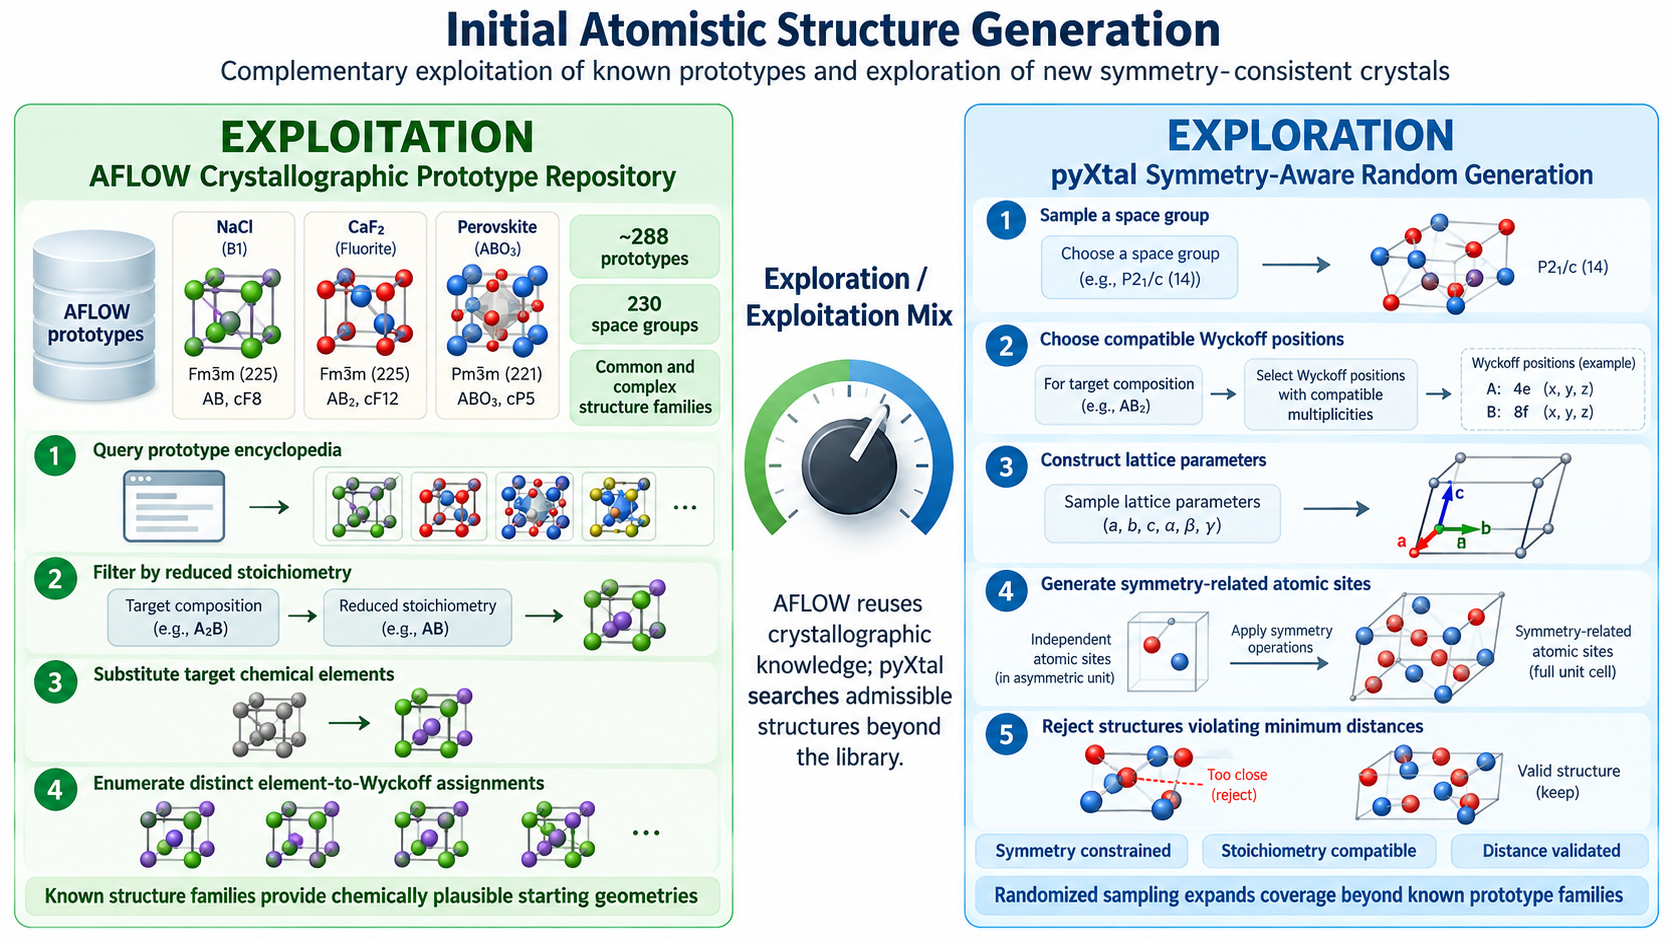
\includegraphics[width=\linewidth]{figures/slide13_panel1.png}
\caption{\textbf{Complementary sources of initial candidate structures.} Known crystallographic prototypes (AFLOW) support exploitation of established structure families, whereas symmetry-constrained randomized generation (PyXtal) supports exploration. Adapted from the authors' presentation (slide 13). These are alternative candidate-generation procedures, not measured comparative discovery yields.}
\label{fig:structure_generation}
\end{figure}

\begin{table}[tb]
\centering
\caption{\textcolor{red!80!black}{Previously reported five-material active-learning campaign statistics, pending reconciliation against raw DFT outputs, convergence records and scheduler accounting. The listed DFT wall times are not verified allocation node-hours or GPU-hours.}}
\label{tab:al}
\resizebox{\columnwidth}{!}{%
\begin{tabular}{lccccccc}
\toprule
System & Nodes & Iters & Cand. & Sel. & Conv. & Fail & \acs{DFT} wall (h)\\
\midrule
Phosphorene (black/blue-P)          & 4 & 8  & 160  & 160  & 160 & 0  & 2.60 \\
LiFePO\textsubscript{4} olivine     & 4 & 10 & 144  & 144  & 144 & 0  & 5.04 \\
CrMnFeCoNi Cantor FCC \acs{HEA}     & 4 & 12 & 433  & 433  & 432 & 1  & 6.17 \\
NbTaVHfZrTi BCC \acs{HEA} & 4 & 5  & 1650 & 1000 & 942 & 58 & 8.42 \\
Zn(HCOO)\textsubscript{2} \acs{MOF} & 4 & 4 & 32 & 32 & 32 & 0 & 0.61 \\
\bottomrule
\end{tabular}%
}
\end{table}

\textcolor{red!80!black}{The reported counts, failures and per-case DFT wall times in Table~\ref{tab:al} remain provisional until the original run outputs and job accounting can be recovered. Application-level elapsed time, summed per-calculation time and scheduler allocation hours must be kept distinct; no allocation cost is inferred from the listed wall-time column.}

The campaign statistics listed in Table~\ref{tab:al} have not yet been reconciled against original calculation records and scheduler logs. If verified, these candidate statistics characterize the acquisition stage across the five
chemistries. For four cases, the number of screened \ac{MD} candidates fell at
or below the per-iteration labeling budget, so essentially every valid frame
was retained. The NbTaVHfZrTi \ac{BCC} \ac{HEA} is the exception: the
\ac{MLIP}-driven sampler generated 1650 valid candidates, from which the
composition-diversity filter selected 1000 for labeling. If the reported counts are confirmed, they are consistent with filtering redundant configurations before higher-fidelity labeling when the sampled set exceeds the labeling budget. The selected structures then become the input to the next stage of
Fig.~\ref{fig:architecture}, first-principles labeling.

\subsubsection{DFT relaxation and MLIP-assisted warm starts}
\label{sec:results:warmstart_setup}
The warm-start experiments address whether \ac{MLIP}
pre-relaxation reduces the effort required by a subsequent \ac{DFT} geometry
optimization, and whether that benefit depends on the selected \ac{MLIP} and
\ac{DFT} backends. This warm-start benchmark is a controlled
ablation of the transition from surrogate evaluation to first-principles
optimization.

\paragraph{Warm-start protocol.}
The warm-start benchmarks are organized as a controlled comparison between two
ways of initializing each first-principles geometry optimization:

\begin{itemize}
\item \textbf{Cold start.} The \ac{DFT} optimizer is launched directly from the
  \emph{original} input coordinates of the fixture, with no \ac{MLIP}
  pre-processing. This is the conventional baseline.
\item \textbf{Warm start.} The same fixture is first relaxed by an \ac{MLIP}
  to $f_\text{max} = 0.01$\,eV/\AA, and the \ac{DFT} optimizer is then launched
  from the \emph{\ac{MLIP}-relaxed} coordinates. The \ac{DFT} settings are held
  identical to the cold run so that any difference in convergence is
  attributable solely to the change of initial geometry.
\end{itemize}

The cold/warm pair is repeated for all four combinations of \ac{MLIP}
pre-relaxer (HydraGNN~\cite{hydragnn} or UMA~\cite{wood2025uma}) and \ac{DFT}
solver (\ac{QE} or \ac{VASP}), a factorial ablation in which varying one factor
at a time attributes any warm-start benefit to the potential, the solver, or
their interaction. Three off-equilibrium alloy fixtures are used---MoNbTaW
\ac{HEA} (16-atom BCC), NbTaW BCC, and NbMoW BCC---each run three times per
backend pairing on Perlmutter; the recorded quantities are the \ac{BFGS}
ionic-step count, per-step and total \ac{SCF} iterations, final energy, and wall
time.

%he three alloy fixtures have random site occupation, so the input geometry carries genuine site-specific forces and the \acs{MLIP} pre-relaxation moves atoms before converging. Each fixture is run under all four backend pairings, giving the twelve rows of Table~\ref{tab:warmstart_matrix}. Each row reports the \acs{BFGS} ionic-step count and total \acs{SCF} iteration count for the cold and warm runs (averaged over three repeats) and the relative change in total \acs{SCF} work, $\Delta_\text{SCF} = (\text{warm}-\text{cold})/\text{cold}$, where negative values indicate a warm-start speed-up. Varying one backend factor at a time isolates whether any benefit comes from the \acs{MLIP} pre-relaxer or the \acs{DFT} solver.

\begin{table*}[tp]
\centering
\caption{Cold vs.\ warm-start convergence for the factorial backend ablation
across the three alloy fixtures.}
\label{tab:warmstart_matrix}
\begin{tabular}{lllcccccc}
\toprule
\multirow{2}{*}{Fixture} & \multirow{2}{*}{\acs{MLIP}} & \multirow{2}{*}{\acs{DFT}}
 & \multicolumn{2}{c}{\acs{BFGS} steps} & \multicolumn{2}{c}{Total \acs{SCF}} & \multirow{2}{*}{$\Delta_\text{SCF}$} & \multirow{2}{*}{Repeats}\\
\cmidrule(lr){4-5}\cmidrule(lr){6-7}
 & & & Cold & Warm & Cold & Warm & & \\
\midrule
\multirow{4}{*}{MoNbTaW \acs{HEA}} & HydraGNN & \acs{QE} & 5 & 5 & 127 & 127 & 0\% & 3 \\
 & HydraGNN & \acs{VASP} & 7 & 7 & 75 & 75 & 0\% & 3 \\
 & UMA & \acs{QE} & 5 & 5 & 127 & 143 & +13\% & 3 \\
 & UMA & \acs{VASP} & 7 & 7 & 75 & 74 & $-$1\% & 3 \\
\cmidrule(lr){1-9}
\multirow{4}{*}{NbTaW BCC} & HydraGNN & \acs{QE} & 5 & 2 & 134 & 224.7 & +68\% & 3 \\
 & HydraGNN & \acs{VASP} & 6 & 6 & 61 & 61 & 0\% & 3 \\
 & UMA & \acs{QE} & 5 & 4 & 134 & 109 & $-$19\% & 3 \\
 & UMA & \acs{VASP} & 6 & 6 & 61 & 56 & $-$8\% & 3 \\
\cmidrule(lr){1-9}
\multirow{4}{*}{NbMoW BCC} & HydraGNN & \acs{QE} & 6 & 6 & 158.3 & 158 & 0\% & 3 \\
 & HydraGNN & \acs{VASP} & 8 & 8 & 76 & 76 & 0\% & 3 \\
 & UMA & \acs{QE} & 6 & 5 & 158 & 141 & $-$11\% & 3 \\
 & UMA & \acs{VASP} & 8 & 5 & 76 & 48 & $-$37\% & 3 \\
\bottomrule
\end{tabular}
\end{table*}

\subsection{Material-specific VASP reference parameterization for E3}
\label{sec:results:e3_vasp_parameterization}
The settings below define a proposed protocol for future E3 reference generation;
they are not settings or results of the historical campaign described above.
E3 will use VASP with PBE-family PAW datasets for all six systems. The historical
PBE single-point calculations and the separate historical Nb--Ta--O Quantum
ESPRESSO records retain their original provenance and are not relabeled or
pooled with these references. Numerical values below are starting specifications
for author review and representative convergence qualification, not evidence of
convergence. PAW datasets define the core--valence representation, whereas PBE
specifies the exchange--correlation approximation; Hubbard $+U$ and dispersion
are additional modeling choices, applied only where physically justified.
Energies from different backends or method signatures (including changes to
functional, PAW dataset, spin setup, $U$, or dispersion) must not be pooled in
an uncorrected reference set or convex hull.

\begin{table*}[htbp]
\centering
\caption{Prospective material-specific VASP reference branches and starting inputs for E3. All settings are candidates for qualification, not completed or converged calculations.}
\label{tab:e3_vasp_parameters}
\scriptsize
\setlength{\tabcolsep}{4pt}
\renewcommand{\arraystretch}{1.12}
\begin{tabularx}{\textwidth}{@{}>{\RaggedRight\arraybackslash}p{0.13\textwidth}>{\RaggedRight\arraybackslash}p{0.22\textwidth}>{\RaggedRight\arraybackslash}p{0.30\textwidth}>{\RaggedRight\arraybackslash}X@{}}
\toprule
Material & Method and correction & Candidate PAW and starting inputs & Required qualification \\
\midrule
LiFePO$_4$ & Spin-polarized PBE+$U$ (Dudarev); Fe $3d$, $U_{\mathrm{eff}}=4.3$\,eV candidate, with 3.5 and 5.0\,eV sensitivity branches. & Li\_sv/Fe\_pv/P/O; \texttt{ENCUT}=650\,eV, \texttt{KSPACING}=0.20\,\AA$^{-1}$, \texttt{ISPIN}=2, Gaussian smearing ($\sigma=0.05$\,eV). & Compare collinear antiferromagnetic orderings and ferromagnetic initialization in a representative cell; retain initial and final site moments. Ground the $U$ choice in independent redox, magnetic, and structural evidence and compare a linear-response estimate where feasible. \\
Cantor FCC alloy & Spin-polarized PBE; no automatic $+U$. & Cr\_pv/Mn\_pv/Fe\_pv/Co\_pv/Ni\_pv; \texttt{ENCUT}=480\,eV, \texttt{KSPACING}=0.20\,\AA$^{-1}$, \texttt{ISPIN}=2, metallic smearing (\texttt{ISMEAR}=1, $\sigma=0.20$\,eV). & Compare magnetic initializations, chemically distinct ordered cells and special quasirandom structures; assess cell-size, volume, and relaxation dependence. \\
NbTaVHfZrTi BCC alloy & PBE baseline without default $+U$; qualify semicore choices for Nb, Ta and other transition metals. & Nb\_pv/Ta\_pv/V\_pv/Hf\_pv/Zr\_sv/Ti\_pv; \texttt{ENCUT}=345\,eV, \texttt{KSPACING}=0.20\,\AA$^{-1}$, nonmagnetic baseline with metallic smearing (\texttt{ISMEAR}=1, $\sigma=0.20$\,eV). & Compare chemical orderings, supercell sizes, and semicore choices. Test spin-polarized starts when moments or independent evidence warrant them; do not constrain relaxations to remain BCC if unstable. \\
Phosphorene & PBE; nonmagnetic baseline unless evidence indicates otherwise. & P; \texttt{ENCUT}=335\,eV, in-plane \texttt{KSPACING}=0.15\,\AA$^{-1}$ and one point normal to the sheet, \texttt{ISPIN}=1, Gaussian smearing ($\sigma=0.05$\,eV). & Qualify vacuum lengths of 18/20/22/25\,\AA and in-plane sampling. Fix the out-of-plane cell during ionic relaxation; compare unstrained structures and $\pm1\%$/$\pm2\%$ in-plane strains. \\
Zn(HCOO)$_2$ metal--organic framework & PBE-D3(BJ) proposed as the reference; verify the meaning of VASP \texttt{IVDW}=12 for the pinned executable version. & Zn/C/H/O; \texttt{ENCUT}=520\,eV, \texttt{KSPACING}=0.20\,\AA$^{-1}$, \texttt{ISPIN}=1, Gaussian smearing ($\sigma=0.05$\,eV). & Compare with PBE without dispersion on a representative subset, but do not mix those energies into the selected reference set. Verify proton orientations, guest occupancy, framework geometry, force/stress and cell-size dependence. \\
Nb--Ta--O & Establish the declared domain with converged PBE and no $+U$; a separate $+U$ branch requires independent physical justification. & Nb\_pv/Ta\_pv/O; \texttt{ENCUT}=520\,eV, \texttt{KSPACING}=0.20\,\AA$^{-1}$; use phase-appropriate spin and smearing, including a triplet oxygen reference. & Qualify standard versus semicore Nb/Ta, reduced-oxide states, magnetic starts, and all predeclared unary/binary/ternary formulas and polymorphs. Never tune $U$ to stabilize a preferred phase. A qualified hull supports stability only within its predeclared, method-compatible domain, not globally exhaustive thermodynamic stability. \\
\bottomrule
\end{tabularx}
\end{table*}

The LiFePO$_4$ $U$ candidate is literature-motivated but not validated for this
campaign; compare it with independent redox, magnetic, and structural evidence
and, where feasible, a linear-response estimate
\cite{dudarev1998,cococcioni2005,wang2006,zhou2004}. D3(BJ) denotes the proposed
Grimme D3 dispersion correction with Becke--Johnson damping
\cite{grimme2010,grimme2011}. Hubbard $+U$ and dispersion are separate
modeling choices, not universal improvements. Changes in functional, PAW
dataset, spin setup, $U$, or dispersion define distinct method signatures;
energies from different signatures or backends must not be pooled in an
uncorrected reference set or convex hull.

\paragraph{Shared controls and convergence qualification.}
For each chosen PAW set, begin cutoff qualification at 1.0, 1.15, 1.30, and
1.40 times the largest component \texttt{ENMAX}; the final cutoff is the lowest
value passing the frozen energy, force, and stress tolerances for every phase
class in that method-specific reference set. Do not carry forward
\texttt{ENCUT}=520\,eV by assumption. Start reciprocal-space qualification at
\texttt{KSPACING}=0.30, 0.25, 0.20, and 0.15\,\AA$^{-1}$ (with a single
point normal to the phosphorene sheet), and test electronic thresholds of
\texttt{EDIFF}=10$^{-5}$, 10$^{-6}$, and 10$^{-7}$\,eV. Compare smearing type
and width for metals and small-gap systems, magnetic initial states where
applicable, and relaxed geometries under successively tighter ionic-force and
residual-stress limits. Proposed acceptance targets are energy changes below
1\,meV/atom, maximum residual force below 0.01\,eV/\AA, and residual stress
below 0.2\,GPa, with stricter hull-energy checks if needed to resolve the
nearest competing phases. These targets must be reviewed and then tested; they
are not achieved results.

The shared explicit starting relaxation inputs are \texttt{GGA=PE},
\texttt{PREC=Accurate}, \texttt{ALGO=Normal}, \texttt{NELM=120},
\texttt{EDIFF}$=10^{-6}$\,eV, \texttt{EDIFFG}$=-0.01$\,eV/\AA,
\texttt{NSW=200}, \texttt{IBRION=2}, \texttt{LASPH=.TRUE.},
\texttt{LREAL=.FALSE.}, and \texttt{ISYM=0}; use \texttt{ISIF=3} for bulk
ion-and-cell relaxation and \texttt{ISIF=2} for phosphorene with the vacuum-axis
cell fixed. Use the per-material spin and smearing starts in
Table~\ref{tab:e3_vasp_parameters}, and record structure-specific
\texttt{MAGMOM}; use
\texttt{LMAXMIX=4} for transition-metal calculations. For fixed-geometry
single-point labels use \texttt{NSW=0} and \texttt{IBRION=-1} with the same
qualified energy-affecting settings. The LiFePO$_4$ Dudarev branch uses
\texttt{LDAU=.TRUE.}, \texttt{LDAUTYPE=2}, and species-ordered
\texttt{LDAUL}, \texttt{LDAUU}, and \texttt{LDAUJ}; the MOF branch uses
\texttt{IVDW=12} only after confirming its meaning for the pinned VASP version.
The rounded starting cutoffs in Table~\ref{tab:e3_vasp_parameters} are
approximately 1.3 times the largest proposed component \texttt{ENMAX} in each
set. They are qualification candidates, not converged values.

Generate geometry-converged structures for reference phases before separate
fixed-geometry single-point labels. Record the full input, ordered species,
PAW component hashes, VASP version, convergence history, magnetic initialization,
and a method signature. The local PAW inventory inspected for planning has no
verified library-release identifier and contains mixed component dates; its
component identities and hashes are an audit snapshot, not authorization or a
claim that the library is homogeneous. The corresponding proposed selections,
component metadata, compatibility rules, and resource-estimation gate are
specified in the run plan. Do not commit or redistribute licensed PAW files.

The completed matrix reveals a clear dependence on the selected backend. On the disordered \ac{BCC}
alloys, UMA-relaxed geometries reduce total \ac{DFT} \ac{SCF} work across
\emph{both} solvers---UMA+\ac{QE} by $19\%$ (NbTaW) and $11\%$ (NbMoW), and
UMA+\ac{VASP} by $8\%$ (NbTaW) and $37\%$ (NbMoW)---whereas HydraGNN
pre-relaxation is neutral on \ac{VASP} ($0\%$ on all three fixtures) and, on
NbTaW+\ac{QE}, \emph{increases} cost ($\Delta_\text{SCF}=+68\%$, with the warm
run exhausting its \ac{SCF} budget without converging). These results show that warm-start performance depends on both the material and the
backend. A change in \ac{SCF} work reflects not only the quality of the
pre-relaxed geometry but also solver conditioning and pseudopotential choice. Because the backend is configurable, the same workflow can switch among potentials or benchmark them on identical fixtures without changing the agentic
orchestration, the \ac{DFT} escalation logic, or the deployment scripts.

\verifyclaim{Warm-start comparisons must report nonconverged runs (including the NbTaW HydraGNN+QE SCF failure) separately from successful-run averages. Audit matched starting geometries, DFT settings, code versions and total wall time; rerun missing MACE/backend combinations only where required for a balanced cross-backend claim. Existing measurements are not a validated claim of universal MLIP warm-start benefit.}


\begin{figure}[t]
\centering
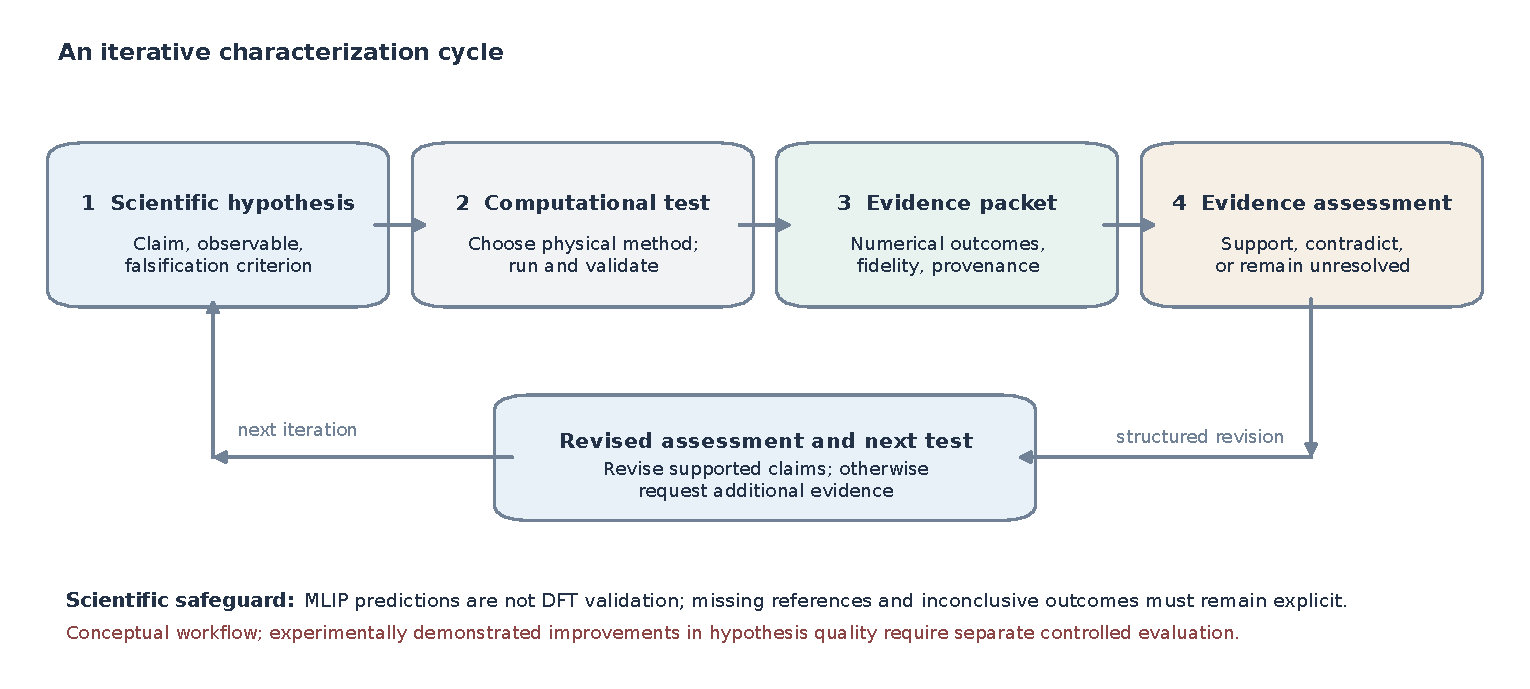
\includegraphics[width=\linewidth]{figures/fig_evidence_cycle_vector.pdf}
\caption{\textbf{Evidence-informed assessment of materials hypotheses.} Hypotheses guide the selection of numerical tests; the resulting observations and their provenance inform the next assessment and, where warranted, additional calculations. The diagram represents scientific interpretation, which is distinct from adapting the interatomic potential.}
\label{fig:evidence_revision}
\end{figure}

\subsubsection{Hypothesis assessment after structural and energetic characterization}
The same evidence packet is supplied to an individual language model and to the multi-model review configuration. The comparison isolates the effect of deliberation from access to additional numerical data and examines whether a modified conclusion is physically supported, contradicted or necessarily unresolved.
The before/after assessment of scientific hypotheses is reported within the E2 fixed-evidence benchmark rather than counted as a separate experiment. For each characterized case, retain the original claim, the complete frozen evidence packet, the policies' initial assessments, the conclusions accepted by the shared validation rules, any justified request for more information, and the scientifically meaningful revision. This separates the value of interpretation from the mechanical protection afforded by the common evidence validator.
\textcolor{red!80!black}{\emph{Results pending:} per-stoichiometry structure/phase characterization and evidence-informed revision across representative hypotheses.}

\subsection{Adaptive characterization at matched DFT budgets}
\label{sec:results_active}
Experiment E3 is a unified, conditional evaluation across the six material systems. Zero-shot HydraGNN, UMA and MACE predictions are assessed for every supported material--model combination against independent reference data, with task-specific acceptance thresholds frozen using validation information only. A supported combination failing these criteria enters the same matched-budget C-versus-D acquisition and model-adaptation pathway, subject to sufficient independent data and documented computational limits. A combination satisfying the criteria retains its pretrained model, although the scientific characterization may still require DFT-level evidence. Combinations lacking adequate validation data are not classified as failures, and unsupported backends are reported explicitly. This experiment evaluates how candidate selection, first-principles labeling and validation-controlled model adaptation affect the reliability and cost of scientific characterization. \ac{DFT} single-point labeling and full geometry relaxation are reported separately because their numerical objectives and costs differ.
For Nb--Ta--O, the scientific investigation includes composition-dependent oxide candidates and the completeness of competing-phase reference information. The repository contains a bounded Nb--Ta--O campaign with multi-LLM discussion, MLIP screening, active learning and Quantum ESPRESSO refinement, but the existence of the campaign configuration does not establish fully converged phase-stability results. Nb--Ta--O reference calculations must therefore be reconciled with their actual outputs, numerical convergence and method-consistent unary and competing oxide phases before acceptance as characterization evidence. The E3 validation gate, C-versus-D acquisition comparison and conditional adaptation rules apply to this sixth system under the same protocol as the other five, with material-specific numerical settings.\par
\subsubsection{HydraGNN, UMA and MACE adaptation and independent prediction errors}
\label{sec:results:finetune}
\paragraph{Materials and paired backend matrix.}
The evaluation encompasses lithium iron phosphate (LiFePO$_4$), a Cantor face-centered-cubic alloy, a NbTaVHfZrTi body-centered-cubic alloy, phosphorene, Zn(HCOO)$_2$ metal--organic framework structures, and Nb--Ta--O compositions and oxide phases. These systems differ in bonding, chemical diversity, dimensionality and expected transfer behavior, making them complementary probes of model adaptation. A common zero-shot evaluation is planned for all supported cells. Each cell is assigned an acceptance status from prespecified validation-only criteria: pass, fail, insufficient validation evidence or unsupported. Fine-tuning and matched-policy adaptive acquisition are applied to failing supported cells, rather than automatically to all cells. Models passing the accuracy criteria remain eligible for scientific DFT validation when required by the question. Final pretrained-versus-adapted comparisons use untouched independent test groups; failures, unavailable backends and infeasible adaptations are reported separately.

\begin{table}[htbp]
\centering\small
\caption{\textcolor{red!80!black}{Planned zero-shot (ZS) evaluations for all supported backend--material combinations. AL/FT denotes conditional active-learning acquisition and fine-tuning only when prespecified validation criteria fail and sufficient data and backend support are available. Results are pending.}}
\label{tab:new_mlip_matrix}
\begin{tabular}{@{}llll@{}}
\toprule
Material & HydraGNN & UMA & MACE \\
\midrule
LiFePO$_4$ & \textcolor{red!80!black}{ZS; AL/FT if needed} & \textcolor{red!80!black}{ZS; AL/FT if needed} & \textcolor{red!80!black}{ZS; AL/FT if needed} \\
Cantor FCC alloy & \textcolor{red!80!black}{ZS; AL/FT if needed} & \textcolor{red!80!black}{ZS; AL/FT if needed} & \textcolor{red!80!black}{ZS; AL/FT if needed} \\
NbTaVHfZrTi BCC alloy & \textcolor{red!80!black}{ZS; AL/FT if needed} & \textcolor{red!80!black}{ZS; AL/FT if needed} & \textcolor{red!80!black}{ZS; AL/FT if needed} \\
Nb--Ta--O oxide system & \textcolor{red!80!black}{ZS; AL/FT if needed} & \textcolor{red!80!black}{ZS; AL/FT if needed} & \textcolor{red!80!black}{ZS; AL/FT if needed} \\
Phosphorene & \textcolor{red!80!black}{ZS; AL/FT if needed} & \textcolor{red!80!black}{ZS; AL/FT if needed} & \textcolor{red!80!black}{ZS; AL/FT if needed} \\
Zn(HCOO)$_2$ MOF & \textcolor{red!80!black}{ZS; AL/FT if needed} & \textcolor{red!80!black}{ZS; AL/FT if needed} & \textcolor{red!80!black}{ZS; AL/FT if needed} \\
\bottomrule
\end{tabular}
\end{table}

\paragraph{Dataset independence and scientific objectives.}
The statistical unit for generalization depends on the scientific question. Configuration-level random partitions can overstate accuracy when temporally correlated molecular-dynamics frames or related starting geometries occur in both training and evaluation sets. The evaluation instead separates trajectories or starting structures and, where supported by the available data, includes composition- or condition-held-out testing. Model selection, reference-energy correction and checkpoint promotion are restricted to training or validation information; independent test configurations remain excluded from these decisions.

\paragraph{Repeatability and comparable adaptation.}
Comparison across HydraGNN, UMA and MACE is based on common physical evidence rather than artificially identical optimization procedures. The relevant observables include energy and force errors, chemically meaningful structural rankings, adaptation and inference expenditure, and variability across independent training initializations. Differences in parameter freezing, low-rank adaptation and model-specific learning strategies are treated as part of the measured computational cost and model behavior. Cross-model disagreement is evaluated against observed first-principles error rather than interpreted as calibrated uncertainty by assumption.

\newexperiment{Staged three-backend interatomic-potential evaluation}{Evaluate zero-shot HydraGNN, UMA and MACE predictions for every supported combination of the six material systems under method-consistent reference conventions and independently grouped validation and test partitions. Determine each cell's acceptance status using prespecified task-specific validation thresholds without examining final test outcomes. For every failing supported cell, apply a bounded, matched-policy acquisition and validation-controlled fine-tuning protocol. Passing cells require no gratuitous retraining; cells with insufficient validation evidence or unsupported backends are documented rather than imputed. Qualify the software pathway on small cases before production without restricting the final material coverage. Report independent-group uncertainty intervals, adapted-versus-incumbent performance, failures and complete training costs; do not select checkpoints on test data.}

\textcolor{red!80!black}{\emph{Results to be inserted:} paired energy and force errors with uncertainty intervals, adaptation cost versus accuracy, in-domain and transfer evaluation, and backend failure statistics.}

\subsubsection{Matched-budget acquisition and sequential characterization}
\label{sec:results:adaptive_policy}
\paragraph{Principal C-versus-D experiment.}
Both policies start from the same initial scientific hypothesis, candidate structure pool, incumbent MLIP, uncertainty information, admissibility rules and reference protocol. Policy C proposes scientific interpretations and follow-up calculations using LLM reasoning; policy D selects follow-up calculations through a prespecified adaptive numerical rule. Decisions are allowed to differ, but the same DFT budget ceiling and numerical execution policy apply. A common cache keyed by atomistic configuration and DFT protocol prevents redundant execution without giving either policy unrequested labels. Each policy is charged for its own requests and failed attempts. A fully labeled pool may be used for preproduction replay only when the policy has no access to unselected labels.

\paragraph{Outcomes and sequential decisions.}
The principal outcome is the fraction of independently assessed scientific questions reaching a justified resolved conclusion as a function of attempted DFT budget. Secondary measures include justified inconclusiveness, unsupported prevalidation claims, missed opportunities for resolution, uncertainty calibration, DFT failures, scientific relevance of selected calculations, and end-to-end computational resource expenditure. The deterministic acquisition policy is a capable uncertainty/diversity-based adaptive baseline, not an intentionally static sequence. A small random-acquisition control may be used as a diagnostic; exhaustive combinations of acquisition rules and uncertainty estimators are not required for the primary claim.

\newexperiment{E3: adaptive characterization and evidence revision}{For every supported material--MLIP cell failing its prespecified validation-accuracy criteria, compare policies C and D with common initial evidence, candidate pools, numerical methods, scientific safeguards, adaptation rules and frozen budgets. First use compatible cached or replayable DFT labels; authorize new DFT calculations only for a specifically missing result. Under both policies, acquire labels, expand datasets, consider fine-tuning when adequate independent training data exist, select models using validation only, and promote candidates only after the same approval criteria. Passing cells remain in the six-system zero-shot evaluation and undergo additional DFT characterization only when evidence requirements demand it. Record task-level resolution-versus-budget curves, acquisition choices, failed and converged calculations, total LLM/MLIP/DFT costs, and whether each new result changes the scientific hypothesis. Repeat on independent tasks/seeds when pilot variance supports a meaningful comparison.}

\subsubsection{Conditional model adaptation and supporting warm-start tests}
Active-learning dataset growth, candidate-model training and model promotion are distinct stages. For each failing supported combination, both C and D apply the same acquisition and adaptation eligibility criteria. Retraining is triggered only if sufficient new independent training data are available and the validation-based accuracy deficit remains; candidate MLIPs are compared with the incumbent on held-out validation groups; the independent test data remain untouched until after model selection. Report prediction error alongside scientifically consequential ranking changes and decisions, rather than treating a reduction in global force MAE as an automatic improvement in characterization.

The direct-DFT versus MLIP-assisted DFT warm-start comparisons already reported in Section~\ref{sec:results:warmstart_setup} remain supporting results. A full post-adaptation warm-start Cartesian product across models, materials and DFT solvers is not mandatory. New runs should be limited to a prespecified subset where adaptation may materially affect relaxation outcomes, and should report final structural and energetic agreement, convergence failures and total cost of both the surrogate and first-principles stages.
\textcolor{red!80!black}{\emph{Results pending:} matched-budget adaptive C-versus-D outcomes for supported failing combinations across all six material systems, budget-normalized scientific resolution curves, and independently evaluated conditional model adaptation.}

\subsection{Cross-architecture portability of scientific characterization (E4)}
\noindent The scientific qualification reported in this section distinguishes a working launcher from a successfully completed characterization. Full facility-environment configuration and launcher specifics are provided in Appendix~\ref{sec:hpc}; supporting throughput and recovery studies are in Appendix~\ref{sec:results_reliability}.
\label{sec:results:crossplatform}
Experiment E4 uses a single bounded common characterization workload rather than repeating the entire materials-by-backend matrix. It evaluates whether the scientific characterization procedure can be executed on OLCF Frontier, ALCF Aurora and NERSC Perlmutter without modifying the characterization objective, evidence-admissibility criteria or decision policy. This supplements, rather than replaces, the scientific comparison of LLM-guided and deterministic adaptive investigations. The existing facility-specific launchers and portability benchmark establish the software mechanisms required for this evaluation; the numerical measurements in the present manuscript are predominantly from Perlmutter. Accordingly, this section does not infer successful end-to-end three-facility execution from the existence of configuration files or launch scripts.

\begin{table}[H]
\centering
\caption{Cross-architecture qualification matrix to be completed using recorded runs. ``Not yet verified'' indicates missing reported end-to-end evidence, not an absence of software support. Platform-specific configurations and scientific criteria must accompany each measured entry.}
\label{tab:cross-platform-qualification}
\small
\begin{tabular}{llll}
\hline
Facility and system & Accelerator ecosystem & MLIP/DFT stages & Full characterization \\
\hline
OLCF Frontier & AMD MI250X / ROCm & \textcolor{red!80!black}{Not yet verified} & \textcolor{red!80!black}{Not yet verified} \\
ALCF Aurora & Intel GPU Max / oneAPI & \textcolor{red!80!black}{Not yet verified} & \textcolor{red!80!black}{Not yet verified} \\
NERSC Perlmutter & NVIDIA A100 / CUDA & Perlmutter runs reported & \textcolor{red!80!black}{Qualify matched contract} \\
\hline
\end{tabular}
\end{table}

\newexperiment{Platform-consistent characterization and resource study}{Complete Table~\ref{tab:cross-platform-qualification} from archived execution logs. For a shared Si or SiC characterization case, report scientific status, relaxation success, final energy per atom, residual forces, structural displacement, DFT ionic/SCF iterations and stage-level walltime and node-hours on each system. Attribute differences from numerical backend, precision or model checkpoint separately from machine effects. Include failures and retried allocations in total cost.}

The primary portability outcome is successful, scientifically consistent execution of a shared characterization procedure across distinct accelerator environments. Stage-level costs characterize practical deployment, but unlike a matched scientific conclusion, an isolated walltime is not directly comparable without documenting the computational resources and numerical methods used. The more extensive Perlmutter throughput, restart and backend-substitution experiments are retained as supporting material in Appendix~\ref{sec:hpc}.

\section{Conclusions and future work}
\label{sec:conclusions}
MATSIM-AGENTS couples scientific hypothesis formulation and evidence assessment to atomistic computation through independently configurable language-model, interatomic-potential, and electronic-structure backends. Its computational architecture allows surrogate predictions and first-principles calculations to be associated with the claims they inform, while persistent execution supports campaigns that extend beyond individual computing allocations. Numerical experiments address candidate exploration, electronic-structure labeling, concurrent computation and checkpointed continuation. The evaluation distinguishes E1a workflow-aligned hypothesis generation from the proposed supplementary E1b cross-domain assessment; E2 evaluates fixed-evidence interpretation, E3 evaluates adaptive evidence acquisition and conditional surrogate adaptation, and E4 evaluates computational portability. These experiments assess different links between hypotheses, evidence, numerical investigation, and execution. No E1a or E1b result is inferred from the framework or design alone. The framework is intended to support material-specific scientific assessments while recognizing that energy ranking, convergence, and thermodynamic stability are distinct physical claims. The deployment layer also provides machine-specific execution paths for the heterogeneous accelerators of OLCF Frontier, ALCF Aurora and NERSC Perlmutter; systematic matched cross-facility qualification remains a separate experimental requirement. Future developments include improved uncertainty calibration, wider chemical coverage and more comprehensive validation of backend interoperability and operational resilience. \textcolor{red!80!black}{[Insert quantitative conclusions only after the corresponding approved experiments have been completed and verified.]}

\section*{Conflicts of interest}
\verifyclaim{All authors must review and approve the final conflicts-of-interest declaration.}
\section*{Data availability}
The open-source framework is available at \url{https://github.com/ORNL/matsim-agents}. \textcolor{red!80!black}{Before submission: provide an immutable code release/commit, dataset DOIs or persistent download links, individual experiment configurations, train/validation/test manifests, model checkpoints where redistributable, and scripts reproducing each reported figure and table. State access restrictions for licensed VASP resources.}
\section*{Acknowledgments}
This work was primarily supported by the Office of Advanced Scientific Computing Research (ASCR) and the Office of Basic Energy Sciences through the SciDAC project ``FORUM-AI: Foundation Models Orchestrating Reasoning Agents to Uncover Materials Advances and Insight'' and by the seed project ``Critical Minerals and Materials to Unlock Supply (CM2US)'' under the Transformational AI Models Consortium (ModCon) initiative of the Genesis Mission. Computing resources were provided by (i) the Oak Ridge Leadership Computing Facility, supported by the DOE Office of Science under the same contract, through American Science Cloud (AmSC) allocation award MAT746 and ASCR Leadership Computing Challenge (ALCC) award LRN070; (ii) the Argonne Leadership Computing Facility, a DOE Office of Science user facility at Argonne National Laboratory, supported by ASCR under contract DE-AC02-06CH11357, through American Science Cloud allocation award CM2US and Director's Discretionary award HydraGNN; and (iii) the National Energy Research Scientific Computing Center (NERSC), a DOE Office of Science user facility, through award ``ScienceAtScale@NERSC'' ASCR-ERCAP0034735 and ASCR-ERCAP0036319.

% =============================================================================

\appendix
\section{Facility-specific execution and resource management details}
\label{sec:hpc}
This appendix expands the architecture-independent resource and execution mechanisms summarized in Section~\ref{sec:methods:portability}. It specifies how backends are deployed without altering the characterization objective or the criteria for scientific evidence. Scientific portability outcomes, rather than installation details, are evaluated in Section~\ref{sec:results:crossplatform}.

\subsection{Platform-agnostic design principles}
\label{sec:hpc:platform_design}
The stack rests on three portability principles. \textbf{Module isolation:} all
\ac{GPU}-software interactions (\ac{CUDA}/\ac{MPI}/compiler toolchain) are
encapsulated behind per-platform shell fragments, so a single function
(\texttt{load\_perlmutter\_modules\_gpu()} or its Frontier/Aurora equivalents)
sets up the environment reproducibly from a clean login shell.
\textbf{Decoupled Python and \ac{MPI} environments:} the \ac{MLIP} backends run
in a PyTorch \ac{GPU} environment, while \ac{QE}/\ac{VASP} require separate
\ac{MPI}/compiler stacks, so the batch script activates the Python environment
for the \ac{MLIP} phase and spawns the \ac{DFT} launcher as a subprocess with
its own compiler/\ac{MPI}/runtime. \textbf{vLLM inference serving:} \ac{LLM}
inference runs in a separate Slurm allocation (or a login-node background process)
behind an OpenAI-compatible \ac{HTTP} endpoint, requiring only the \texttt{openai}
package on the client side. The first-principles code is exposed as a
user-selectable backend (\ac{QE} or \ac{VASP}); the repository ships build and
launch scripts for both on Perlmutter, Frontier, and Aurora, documenting the
module loads, compiler choices, \ac{MPI}/offload settings, and launcher
conventions each system requires, while \ac{VASP} users must supply their own
licensed source and pseudopotentials.

\subsection{Facility-specific deployment}
\label{sec:hpc:platform_deployment}
The framework is built and deployed on all three \ac{DOE} leadership-class
systems, each with a distinct accelerator and \ac{DFT} offload backend
(Perlmutter/NVIDIA A100 via NVHPC \ac{CUDA}, Frontier/AMD MI250X via HIP OpenMP
target offload, Aurora/Intel \ac{PVC} via OneAPI); the per-platform module
loads, compiler choices, and offload settings live in the released build scripts.


% =============================================================================
% =============================================================================



% Supporting performance and interoperability analyses are included in the appendix.
\section{Supporting numerical performance and interoperability studies}
\label{sec:appendix:performance}
The main characterization comparisons are defined in Section~\ref{sec:results_protocol} and reported in Section~\ref{sec:numerical_results}. This appendix collects additional qualification tests and technical performance results required to assess backend interchangeability, execution overhead, recovery and resource consumption, without treating those implementation metrics as substitutes for scientifically correct conclusions.
\subsection{Codabench-compatible evaluation of interatomic potentials}
\label{sec:appendix:codabench}
The repository includes a Codabench competition definition and scoring interface in
\texttt{benchmarks/codabench/}. A submission may provide formation energies per atom,
per-atom Cartesian forces, relaxed structures, structures and energies from
MLIP-assisted DFT relaxation, and formation energies for fixed-composition ranking.
The corresponding evaluations are formation-energy mean absolute error in
eV/atom, force-component mean absolute error in eV/\AA, relaxed-structure
root-mean-square displacement in \AA, both geometric and energetic errors for
MLIP-assisted DFT relaxation, and mean Spearman rank correlation within
composition groups. Scores for individual tasks are reported alongside an
aggregate normalized score; the latter should not replace task-specific
accuracy when selecting a potential for a scientific investigation.

The competition configuration specifies a deterministic, formula-stratified
public/private partition (\texttt{SEED=42}, public fraction 0.30) and identifies
37 public and 84 private structures among the 121 completed reference labels
described in that configuration. These counts describe the packaged benchmark
configuration, not a completed multi-model evaluation. Compound identities
are withheld behind opaque structure identifiers. The submission protocol
requires consistent formation-energy references: each MLIP uses its own
elemental predictions to form its formation energies, while DFT reference
labels use method-consistent DFT elemental energies. Compound DFT predictions
are not admissible as MLIP submissions.

This benchmark evaluates the underlying numerical surrogate and its
relaxation-related outputs independently of the agentic decision policy.
In particular, low errors on energies and forces, or a high within-composition
ranking correlation, do not imply calibrated uncertainty or establish
thermodynamic stability relative to a complete convex hull.
Backend comparisons should therefore use common structures and
reference conventions, explicitly report failed calculations and
task-level metrics, and retain group-independent train/validation/test
partitions when model adaptation is assessed. The executable benchmark
specification documents the scoring protocol; any model-specific numerical
results require separately executed and verified submissions.

\subsection{Scientific interoperability across LLM, MLIP and DFT backends}
\label{sec:results_interoperability}
\newexperiment{LLM backend sensitivity on common characterization tasks}{Run at least one local LLM and one hosted-service LLM against the same held-out replay and live characterization tasks. Fix tool availability and scientific evidence, document versions and decoding settings, and report conclusion correctness, unsupported claims, tool-call validity, inference latency and token cost. Use multiple runs per model to measure outcome variability.}
The standardized Codabench-compatible tasks provide an additional, policy-independent view of surrogate quality; their definitions and reference conventions are given in Appendix~\ref{sec:appendix:codabench}.
\newexperiment{MLIP backend sensitivity and cross-model disagreement}{Evaluate HydraGNN, UMA and MACE on identical independent DFT-labelled structures and report comparable force/energy errors, within-composition rankings, failed relaxations and cost. Test whether disagreement predicts actual errors; do not interpret agreement as independent physical validation.}
\label{sec:systems_results}
Scientific backend interchangeability and facility portability are enabling contributions. They are evaluated here as separate questions, so as not to conflate support for an interface, successful end-to-end execution, and validated numerical or performance equivalence.
\subsection{Computational throughput, restart and portability}
\label{sec:results_reliability}
\subsubsection{DFT evidence-generation throughput and scaling}
\label{sec:results:scaling}
The selected candidates from the preceding stage are labeled by concurrent
single-point \ac{DFT} calculations. Across the five campaigns, the workflow
dispatched jobs within a four-node allocation (four one-node \ac{VASP} jobs at
a time, or two two-node jobs for the denser Zn(HCOO)\textsubscript{2}
framework). As reported in Table~\ref{tab:al}, \ac{DFT} convergence exceeded
94\% in every case and reached 100\% for phosphorene and
LiFePO\textsubscript{4}. This high convergence rate provides an additional check
that the preceding \ac{MLIP} exploration and screening stages supply
physically usable configurations to the first-principles backend.

\begin{figure}[tb]
\centering
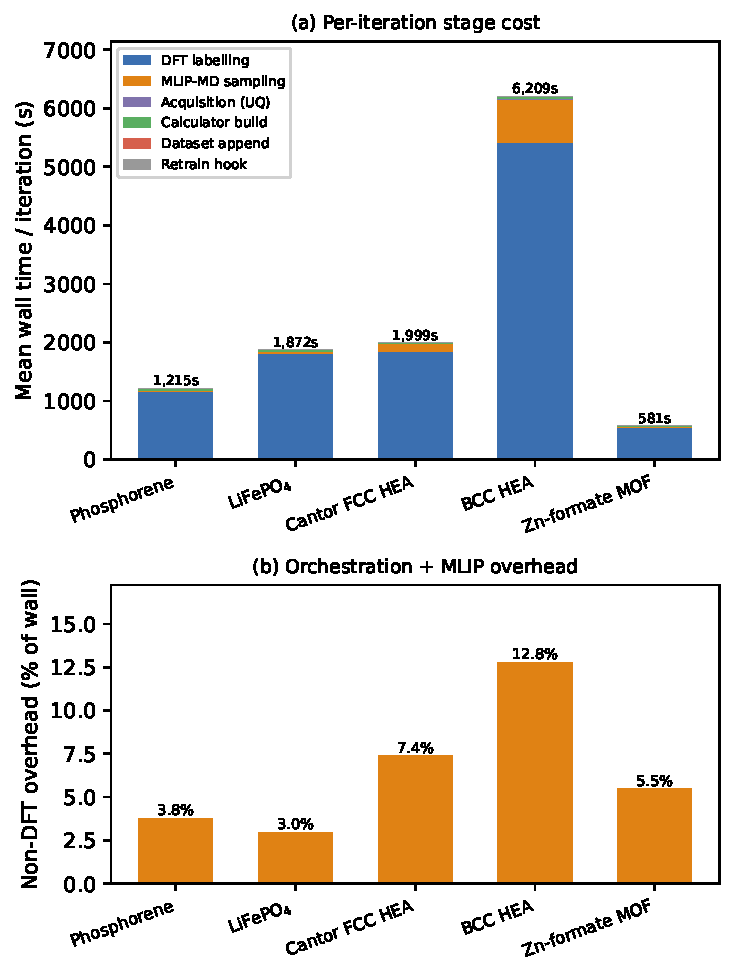
\includegraphics[width=\columnwidth]{figures/al_timing_breakdown.pdf}
\caption{Per-iteration wall-time breakdown of the \acs{AL} loop across
the five test cases. (a) Mean wall time per iteration, stacked by stage.
(b) Combined non-\ac{DFT} time (calculator construction, \ac{MLIP}-\ac{MD}
sampling, candidate acquisition, dataset append, and the retrain hook) as a
percentage of iteration wall time.}
\label{fig:al_timing}
\end{figure}

Figure~\ref{fig:al_timing} decomposes the per-iteration wall time by stage.
Single-point \ac{DFT} labeling accounts for 88--97\% of the wall clock in
every case, while all non-\ac{DFT} stages combined---building the
\ac{MLIP} calculator, running the Langevin \ac{MD} sampler, selecting
candidates by the composition-diversity filter, appending the labeled frames, and invoking the
retrain hook---contribute only 3--12\%. The acquisition and dataset-management
stages are sub-second to a few seconds per iteration (e.g.\ 2.6\,s acquisition
and 0.15\,s append for the Cantor \ac{HEA}); the only non-trivial non-DFT cost
is \ac{MLIP}-\ac{MD} sampling, which scales with system size and step count.
The aggregate non-\ac{DFT} cost remains small relative to first-principles
labeling, so \ac{DFT} remains the dominant computational cost of the workflow.

Because single-point \ac{DFT} labeling is the dominant computational stage, we
next evaluate its strong scaling before proceeding to dataset update and model
adaptation. A fixed 32-frame workload of FCC \ac{HEA} configurations, drawn
from CrMnFeCoNi and four near-equimolar FCC compositions, was labeled by
single-point \ac{VASP} at $N\in\{1,2,4,8\}$ nodes. At node count $N$, the
workload is processed by $N$ simultaneous one-node \ac{VASP} jobs (four A100
ranks each), so the same 32 frames are evaluated with $N$-way parallelism.
Because the workload remains fixed as the number of nodes increases, this is a
strong-scaling measurement.

To quantify variability across workload draws, we repeated the sweep $R=5$
times. Each repeat used an independent random 32-frame workload that was held
fixed across node counts. Throughput was measured from in-job timers as
converged frames per \ac{DFT}-hour
($\text{throughput}=n_\text{conv}/t_\text{DFT}\times3600$), independent of
scheduling latency, and parallel efficiency was defined as
$100\times(\text{throughput}_N/N)/\text{throughput}_1$ relative to the
single-node baseline.

\begin{figure}[tb]
\centering
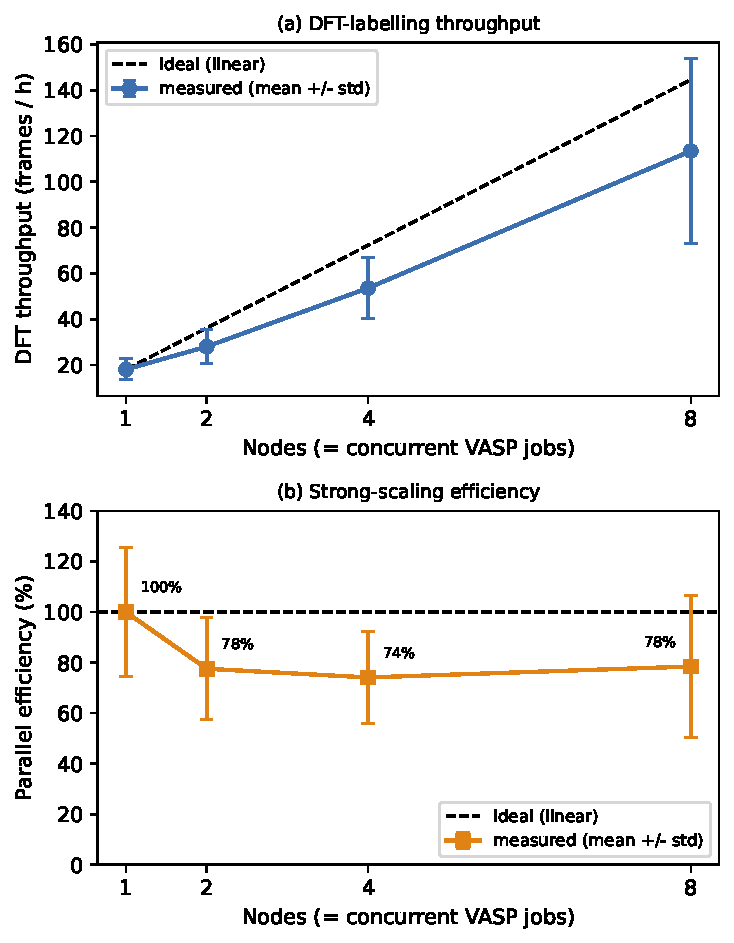
\includegraphics[width=\columnwidth]{figures/al_dft_scaling.pdf}
\caption{Strong scaling of the \acs{DFT}-labeling stage on Perlmutter: a fixed
32-frame FCC \ac{HEA} workload labeled with $N$-way single-point \ac{VASP}
concurrency ($N\in\{1,2,4,8\}$ one-node jobs, four A100 ranks each).
(a) Work-normalized \ac{DFT} throughput (converged frames per \ac{DFT}-hour)
and (b) parallel efficiency vs.\ node count, each averaged over $R=5$ randomized
workload draws with $\pm$ one standard deviation error bars; the dashed line is
the ideal-linear reference.}
\label{fig:al_dft_scaling}
\end{figure}

Figure~\ref{fig:al_dft_scaling} reports the mean throughput and parallel
efficiency over the five repeats. Throughput rises from $18.1\pm4.6$ frames/h on
one node to $28.0\pm7.3$ (two nodes), $53.6\pm13.3$ (four nodes), and
$113.5\pm40.5$ (eight nodes), corresponding to speedups of $1.55\times$,
$2.96\times$, and $6.28\times$. Parallel efficiency remains between 74\% and
79\% across the scaled runs.

The residual sublinear scaling arises primarily from variability within the \emph{fixed} workload:
random alloy frames differ widely in \ac{SCF} difficulty, so at high concurrency
the makespan is determined by the slowest frame in a repeat (enlarging the workload from $16$ to $32$ frames raises eight-node
throughput from $66.9$ to $113.5$ frames/h). The embarrassingly parallel
\ac{DFT}-labeling workload thus retains approximately $74$--$79\%$ parallel
efficiency up to eight concurrent nodes.

The converged first-principles frames produced by this stage are appended to the
case-specific datasets and provide the training data for the next stage of the
workflow.

\subsubsection{Restart across allocation boundaries and limits of portability evidence}
\label{sec:results:portability}
The workflow-level results above also test two cross-cutting systems properties
that are not associated with a single scientific-computation box in
Fig.~\ref{fig:architecture}: recovery across batch-allocation boundaries and
portability across scientific backends and computing platforms.

Across all five campaigns, the complete sequence from \ac{MLIP} exploration
through dataset update executed without manual intervention. The workflow is
also resilient to the wall-time limits common in shared \ac{HPC} environments:
state is checkpointed after every iteration through a per-iteration
\texttt{state.json} file together with the growing \texttt{dataset.extxyz}, so a
job that is pre-empted or reaches its wall-time limit can resume from the last
completed iteration without manual bookkeeping. The LiFePO\textsubscript{4}
campaign in Table~\ref{tab:al} provides a concrete checkpoint/restart test. It
was interrupted by the wall-time limit after five iterations and resumed in a
second allocation to complete the remaining five while reusing all previously
labeled frames. This behavior validates the checkpointed state machine and
allows long-running campaigns to span multiple, potentially backfill-friendly,
batch allocations without reconstructing workflow state manually.

%The loop treats both the \acs{MLIP} and the first-principles engine as configuration-selected backends rather than hard-coded dependencies, so the same orchestration targets different accelerators and \acs{DFT} codes without code changes. On Perlmutter the identical phosphorene loop labels structures with either \acs{VASP} or \acs{QE} by changing only the \texttt{dft:} block of the configuration; each code is reached through a thin per-platform launcher that performs its own module swap, avoiding conflicts between the driver's Python/\acs{MLIP} environment and the \acs{DFT} code's compiler/\acs{MPI} stack. HydraGNN builds on all three target accelerators and both \acs{QE} and \acs{VASP} compile on all three facilities (Section~\ref{sec:hpc}), but end-to-end campaigns with reported measurements are reported only on Perlmutter. The framework is therefore portable by design, with performance measurements currently reported for Perlmutter.

%Taken together, these experiments close the loop back to Fig.~\ref{fig:architecture}: \acs{MLIP} exploration generates candidate configurations, the acquisition stage selects configurations for \acs{DFT}, the first-principles backend provides labels, those labels update and adapt the surrogate, and the measured post-adaptation accuracy informs the evidence gate. The warm-start, checkpoint/restart, and portability studies complement this stage-by-stage validation by quantifying backend sensitivity and the systems properties required for unattended execution on leadership-class \acs{HPC}.


\subsubsection{Controlled end-to-end backend substitution}
Backend substitution is scientifically meaningful only when the characterization objective, observables and physical approximations remain comparable. For electronic-structure calculations, the exchange--correlation treatment, pseudopotentials, magnetic assumptions, numerical convergence and reference-energy conventions determine the interpretation of cross-code results. In particular, raw absolute energies from distinct first-principles implementations are not automatically commensurable.

The present results use VASP for complete campaigns and include separate QE warm-start cases. The ability to choose QE in a configuration does not itself establish a successful matched, complete-loop experiment.
\newexperiment{Complete-loop DFT and MLIP substitution}{Run a matched small workflow with VASP and QE, and with at least two MLIP backends, retaining scientific inputs and acceptance criteria while documenting backend-dependent numerical parameters. Report outcomes, method comparability and overhead.}

\subsubsection{Cross-facility functional qualification and performance limits}
\newexperiment{Real compute across facilities}{Distinguish contract/mocked portability tests from actual MLIP and QE/VASP calculations on Perlmutter, Frontier and Aurora. Record exact code/configuration versions, valid scientific outputs and resource costs. If not performed, restrict claims to deployment support.}
\newexperiment{Failure injection and honest overhead}{Interrupt DFT execution, partial dataset writes and model promotion; assess duplicate prevention, result consistency and recovery overhead. Report allocation-boundary resumption separately from fault-injection recovery.}
\subsection{Integrated cost-accounting considerations}
\label{sec:results_synthesis}
The integrated assessment relates the reliability of characterization decisions to the physical fidelity and cost of the evidence on which those decisions depend. Comparison with fixed and adaptive deterministic workflows is necessary to attribute any incremental benefit to language-model reasoning rather than established numerical selection strategies. Likewise, a decrease in surrogate prediction error matters to the present scientific objective only insofar as it improves the subsequent characterization or reduces the cost of obtaining an adequately supported conclusion.
\newexperiment{Results synthesis and claim validation}{Report the C-versus-D characterization comparison at matched budgets, with shared evidence validation in both policies, together with the three-backend model-adaptation study, and a per-material audit of scientific conclusions and costs.}


\bibliographystyle{unsrtnat}
\bibliography{references}
\end{document}
